\documentclass{beamer}
%\usetheme{Boadilla}
%\usetheme{Szeged}
%\usetheme{Singapore}
%\usetheme{Frankfurt}
\usecolortheme{dove}
%\setbeamertemplate{navigation symbols}{{\footnotesize\insertframenumber}}
\setbeamertemplate{navigation symbols}{}
%\setbeamertemplate{headline}{%
  %  \leavevmode%
    %\hbox{%
    %\insertsectionnavigationhorizontal{\textwidth}{\hspace{20pt}}{\hspace{20pt}}
  %}
%}
\newenvironment{alltt}{\ttfamily}{\par}
\usepackage{amsmath,amssymb,amsfonts,amsthm, multicol, subfigure, color}
\usepackage{bm}
\usepackage{graphicx}
\usepackage{tabularx}
\usepackage{booktabs}
\usepackage{hyperref}
\usepackage{pdfpages}
\usepackage{xcolor}
\definecolor{dodgerblue}{rgb}{.118, .575, 1}
\definecolor{seagreen4}{RGB}{46, 139, 87}
\def\independenT#1#2{\mathrel{\rlap{$#1#2$}\mkern2mu{#1#2}}}
\newcommand\independent{\protect\mathpalette{\protect\independenT}{\perp}}
\newcommand\indep{\protect\mathpalette{\protect\independenT}{\perp}}
\def\logit{\text{logit}}
\usepackage{stackrel}
\usepackage{tikz}
\usetikzlibrary{arrows,shapes.arrows,positioning,shapes,patterns,calc,snakes}
\newcommand\slideref[1]{\vskip .1cm \scriptsize \textcolor{gray}{{#1}}}
\newcommand\red[1]{{\color{red}#1}}
\newcommand\bred[1]{{\color{red}\textbf{#1}}}
\newcommand\blue[1]{{\color{blue}#1}}
\newcommand\bblue[1]{{\color{blue}\textbf{#1}}}
\newcommand\gray[1]{{\color{gray}#1}}
\newcommand\bgray[1]{{\color{gray}\textbf{#1}}}
\newcommand\green[1]{{\color{seagreen4}#1}}
\newcommand\bgreen[1]{{\color{seagreen4}\textbf{#1}}}
\newcommand\purple[1]{{\color{purple}#1}}
\newcommand\orange[1]{{\color{orange}#1}}
\newcommand\black[1]{{\color{black}#1}}
\newcommand\white[1]{{\color{white}#1}}
\newcommand\teal[1]{{\color{teal}#1}}
\newcommand\magenta[1]{{\color{magenta}#1}}
\newcommand\Fuchsia[1]{{\color{Fuchsia}#1}}
\newcommand\BlueGreen[1]{{\color{BlueGreen}#1}}
\colorlet{lightgray}{gray!40}
\pgfdeclarelayer{bg}    % declare background layer for tikz
\pgfsetlayers{bg,main} % order layers for tikz
\newcommand\mycite[1]{\begin{scriptsize}\textcolor{darkgray}{(#1)}\end{scriptsize}}
\newcommand\iid{\stackrel{\text{iid}}{\sim}}
\newcommand\E{\text{E}}
\newcommand\V{\text{V}}
\renewcommand\P{\text{P}}
\newcommand{\Cov}{\text{Cov}}
\newcommand{\Cor}{\text{Cor}}
\newcommand\doop{\text{do}}
\newcommand{\tcframe}{\frame{
\small{
\only<1|handout:0>{\tableofcontents}
\only<2|handout:1>{\tableofcontents[currentsection]}}
}}
% Credit for the following to https://tex.stackexchange.com/questions/44983/beamer-removing-headline-and-its-space-on-a-single-frame-for-plan-but-keepin
\makeatletter
    \newenvironment{withoutheadline}{
        \setbeamertemplate{headline}[default]
        \def\beamer@entrycode{\vspace*{-\headheight}}
    }{}
\makeatother
\setbeamercovered{invisible}
\usepackage[round]{natbib}
\bibliographystyle{humannat-mod}
\setbeamertemplate{enumerate items}[default]
\usepackage{mathtools}
% BELOW THREE LINES MAKES NAME IN FOOTER
\setbeamertemplate{footline}[text line]{%
%\parbox{\linewidth}{\vspace*{-8pt}Ian Lundberg (Princeton)}}
%\parbox{\linewidth}{\vspace*{-8pt}Ian Lundberg. Prediction in Social Science.\insertsectionnavigationhorizontal{.6\paperwidth}{}{\hfill\hfill}}}
\parbox{\linewidth}{\vspace*{-8pt}\bgray{Ian Lundberg} \insertsectionnavigationhorizontal{.75\paperwidth}{}{\hfill\hfill}}}
%\hfill \insertframenumber/23}}%\hfill\insertshortauthor\hfill\insertpagenumber}}
%\setbeamertemplate{navigation symbols}{}
\usepackage{framed}
\usepackage{soul}
\usepackage{appendixnumberbeamer}

\newcommand{\roadmap}[5]{
\begin{frame}
\begin{tikzpicture}[x = \textwidth, y = .9\textheight]
\node at (0,0) {};
\node at (1,1) {};
\node[anchor = north west, font = \Large] at (0,1) {\bgray{Prediction in Social Science}};
\node[anchor = north west] at (0, .92) {A Tool to Study Inequality in Populations};
\node[anchor = north west, font = \small] at (0, .75) {Three possible uses:};
\node[anchor = north west, font = \small] at (0.05,.67) {1)};
\node[anchor = north west, font = \small] at (0.05,.59) {2)};
\node[anchor = north west, font = \small] at (0.05,.51) {3)};
\node[anchor = north west, font = \small] at (.1,.67) {Prediction for individuals};
\node[anchor = north west, align = left, font = \small] at (.1,.59) {Prediction for description};
\node[anchor = north west, align = left, font = \small] at (.1,.51) {Prediction for causal claims};
\node[anchor = north east, font = \small] at (1,.67) {very hard};
\node[anchor = north east, font = \small] at (1,.59) {useful};
\node[anchor = north east, font = \small, align = right] at (1,.51) {opportunities\\abound};
\node[anchor = north west, font = \footnotesize, align = left] at (.1, .43) {--- Define the intervention};
\node[anchor = north west, font = \footnotesize, align = left] at (.1, .38) {--- Causal assumptions};
\node[anchor = north west, font = \footnotesize, align = left] at (.1, .33) {--- Estimation};
\node[anchor = north west, font = \footnotesize, align = left] at (.1, .28) {--- Empirical examples};
\draw[->, line width = 2pt, #1] (#2,#3) -- (#4,#5);
\end{tikzpicture}
\end{frame}
}

\title{Prediction in Social Science}
\author{Ian Lundberg}
\date{\today}

\begin{document}

%{
%\setbeamertemplate{footline}[text line]{\parbox{\linewidth}{\vspace*{-8pt}Ian Lundberg\hfill\insertsection}}

\begin{frame}
\begin{tikzpicture}[x = \textwidth, y = \textheight]
\node at (0,0) {};
\node at (1,1) {};
\node[anchor = north west, align = left, font = \LARGE] at (0,.9) {Prediction in Social Science};
\node[anchor = north west, align = left, font = \Large] at (0,.8) {A Tool to Study Inequality in Populations};
% At top right
%\node[anchor = north east, align = right, font = \Large] at (1,.6) {\bgray{Ian Lundberg}};
%\node[anchor = north east, align = right, font = \footnotesize] at (1,.5) {Princeton University\\Department of Sociology\\ilundberg@princeton.edu};
% At bottom left
\node[anchor = north, align = center, font = \Large] at (.5,.65) {\bgray{Ian Lundberg}};
\node[anchor = south, align = center, font = \footnotesize] at (.5,.38) {University of California, Los Angeles\\Department of Sociology\\California Center for Population Research\\ianlundberg@ucla.edu};
\node[anchor = north, align = center, font = \small] at (.5,.37) {5 October 2021\\University of Wisconsin, Madison\\Center for Demography and Ecology Seminar};
%\node[anchor = south, align = center, font = \footnotesize] at (.5,.33) {Princeton University\\Department of Sociology\\ilundberg@princeton.edu};
\node[anchor = south west, align = left, font = \tiny, text width = \textwidth] at (0,.1) {Replication code is available in links on my CV at ianlundberg.org. Research reported in this talk was supported by The Eunice Kennedy Shriver National Institute of Child Health \& Human Development of the National Institutes of Health under Award Number P2CHD047879, and by the Russell Sage Foundation.};
\end{tikzpicture}
\end{frame}

\begin{frame}
\begin{tikzpicture}[x = \textwidth, y = .9\textheight]
\node at (0,0) {};
\node at (1,1) {};
\node[anchor = north west, font = \Large] at (0,1) {\bgray{Prediction in Social Science}};
\node[anchor = north west] at (0, .92) {A Tool to Study Inequality in Populations};
\node<2->[anchor = north west, font = \small] at (0, .75) {Three possible uses:};
\node<3->[anchor = north west, font = \small] at (0.05,.67) {1)};
\node<5->[anchor = north west, font = \small] at (0.05,.59) {2)};
\node<7->[anchor = north west, font = \small] at (0.05,.51) {3)};
\node<3->[anchor = north west, font = \small] at (.1,.67) {Prediction for individuals};
\node<5->[anchor = north west, align = left, font = \small] at (.1,.59) {Prediction for description};
\node<7->[anchor = north west, align = left, font = \small] at (.1,.51) {Prediction for causal claims};
\node<4->[anchor = north east, font = \small] at (1,.67) {very hard};
\node<6->[anchor = north east, font = \small] at (1,.59) {useful};
\node<8->[anchor = north east, font = \small, align = right] at (1,.51) {opportunities\\abound};
\node<9->[anchor = north west, font = \footnotesize, align = left] at (.1, .43) {--- Define the intervention};
\node<9->[anchor = north west, font = \footnotesize, align = left] at (.1, .38) {--- Causal assumptions};
\node<9->[anchor = north west, font = \footnotesize, align = left] at (.1, .33) {--- Estimation};
\node<9->[anchor = north west, font = \footnotesize, align = left] at (.1, .28) {--- Empirical examples};
\end{tikzpicture}
\end{frame}

\section{Prediction for Individuals.}

\roadmap{blue}{0}{.637}{0.04}{.637}

\begin{frame}
\begin{tikzpicture}[x = \textwidth, y = .9\textheight]
\node at (0,0) {};
\node at (1,1) {};
%\node[anchor = north west, font = \large] at (0,1) {Prediction};
\node[anchor = west, font = \bf, color = gray] at (0,.9) {Standard prediction setting};
\node[anchor = east] at (.35,.7) {\includegraphics[width = .25\textwidth]{figures/20061107apple.jpg}};
\node<2-7>[anchor = west] at (.65,.7) {Apple};
\draw<2->[->, line width = 2pt] (.4,.7) -- (.6,.7);
\node<3> at (.5,.3) {\includegraphics[width = .5\textwidth]{figures/apple_search}};
\node<4->[anchor = west, font = \bf, color = gray] at (0,.45) {Social settings};
\node<4->[anchor = east] at (.35,.35) {Social Data};
\node<4->[anchor = west] at (.65,.35) {Social Outcome};
\draw<4->[->, line width = 2pt] (.4,.35) to node[midway, above] {?} (.6,.35);
\node<5> at (.5,.6) {\includegraphics[width = \textwidth]{figures/nytimes_cps}};
\node<6> at (.5,.6) {\includegraphics[width = \textwidth]{figures/propublica_compas}};
%\node<11->[align = center] at (.5,.15) {These settings are \bblue{distinct} in important ways};
\end{tikzpicture}
\end{frame}

% PREDICTION FOR INDIVIDUALS

\begin{frame}
\includegraphics[width = \textwidth, trim = {0 6.5in 0 .6in}, clip]{figures/pnas_page1}
\end{frame}

\begin{frame}

\centering
\begin{tikzpicture}[x = \textwidth, y = \textheight]
\node at (0,0) {};
\node at (1,1) {};
% Life course visualization
%\draw[->, line width = 2pt, gray] (.2,.85) -- (.8,.85);
%\node[anchor = south] at (.5,.85) {Life course};
%\node[anchor = north west, font = \footnotesize, align  = left] at (.2,.85) {Early\\experiences};
%\node[anchor = north east, font = \footnotesize, align  = right] at (.8,.85) {Later\\outcomes};
\node<1-> at (.5,.8) {\includegraphics[width=\textwidth]{figures/ff_logo}};
% Illustration in data format
%\node<3-10>[anchor = south, font = {\footnotesize\bf}] at (.35, .35) {Predictor variables};
%\node<3-10>[anchor = south, font = {\footnotesize\bf}, rotate = 90] at (.1, .225) {Cases};
\node<2>[anchor = south, font = {\footnotesize\bf}] at (.35, .35) {Predictor variables};
\node<2>[anchor = south, font = {\footnotesize\bf}, rotate = 90] at (.1, .225) {Cases};
\node<3->[anchor = south, font = {\footnotesize\bf}] at (.35, .35) {Predictor variables (12,942)};
\node<3->[anchor = south, font = {\footnotesize\bf}, rotate = 90] at (.1, .225) {Cases (4,242)};
\draw<2->[rounded corners] (.1, .1) rectangle (.6,.35);
\node<2->[anchor = south, font = {\footnotesize\bf}] at (.8, .35) {Outcomes};
\draw<2-4>[rounded corners] (.7, .1) rectangle (.9,.35);
\draw<2->[->, line width = 4pt, gray] (.62, .225) -- (.68,.225);
% Analogy to the apple task
\node<2> at (.35,.225) {\includegraphics[width = .25\textwidth]{figures/20061107apple.jpg}};
\node<2-3> at (.8,.225) {Apple};
% Introduce FF
%\node<2>[font = \footnotesize, align = center] at (.35,.225) {Early Life Experiences};
%\node<2>[font = \footnotesize, align = center] at (.8,.225) {Later Life\\Outcomes};
\node<3->[font = \footnotesize, align = center] at (.35,.225) {Childhood Experiences\\Birth to age 9};
\node<4>[font = \footnotesize, align = center] at (.8,.225) {GPA\\Age 15};
% Numeric details of the task
\draw<5->[fill = gray, rounded corners] (.7,.1) rectangle (.9,.225);
\draw<5->[rounded corners] (.7,.225) rectangle (.9,.35);
\node<5->[font = \footnotesize, align = center] at (.8,.2875) {GPA\\Age 15};
\node<5->[font = \footnotesize, align = center, white] at (.8,.1625) {GPA\\Age 15};
\node<5->[rotate = 270, anchor = south, font = {\footnotesize}, align = center] at (.9,.2875) {\textbf{Train}};
\node<5->[rotate = 270, anchor = south, font = {\footnotesize}, align = center] at (.9,.1625) {\textbf{Holdout}};
\node<6->[align = left, anchor = west, font = {\bf}, gray] at (.15,.6) {Mass collaboration};
\node<6->[font = \small, align = left, anchor = west] at (.15,.55) {160 teams attempted this task};
\end{tikzpicture}
\end{frame}

\begin{frame}{The best of 160 submissions}
\begin{center}
\begin{tikzpicture}[x = \textwidth, y = \textheight]
\node at (0,.5) {};
\node at (1,.5) {};
\node<1> at (.3,.55) {\includegraphics[height = .7\textheight]{figures/gpa_best_scatter_diagonal_flipped_nodots}};
\node<2-> at (.3,.55) {\includegraphics[height = .7\textheight]{figures/gpa_best_scatter_diagonal_flipped}};
\node<3->[anchor = east, align = left, font = \small, outer sep = 10pt] (variability) at (1,.6) {At any\\predicted GPA,\\the true GPA\\varies tremendously};
\draw<3->[<->, thick] (variability.south west) -- (variability.north west);
\draw<4>[fill = gray, fill opacity = .2, draw = white, rounded corners] (.27,.31) rectangle (.45,.44);
\end{tikzpicture}
\end{center}
\end{frame}

%%%%%%%%%%%%%%%%%%%%%%%%%%%
\begin{frame}
\centering
\begin{tikzpicture}[x = \textwidth, y = \textheight]
\node<1>[anchor = north] at (.5,1) {\includegraphics[width=.9\textwidth]{figures/image1_GPA_only}};
\node<2>[anchor = north] at (.5,1) {\includegraphics[width=.9\textwidth]{figures/image1}};
%\node<3>[anchor = north] at (.5,1) {\includegraphics[width=.9\textwidth]{figures/image1a}};
\end{tikzpicture}
\end{frame}

%%%%%%%%%%%%%%%%%%%%%%%%%%%
\begin{frame}
\begin{tikzpicture}[x = \textwidth, y = .9\textheight]
\node at (0,0) {};
\node at (1,1) {};
\node<1->[align = center, font = \large] at (.5,.8) {Machine learning was \\\bblue{really bad}\\at predicting individual outcomes in this social setting};
%%%%
% Highlight MSE .3 to .4 was the exact vertical height
\draw<5>[fill = gray, draw = white, fill opacity = .1, rounded corners] (.07,.2) rectangle (.29,.41);
% Highlight conditional variance
\draw<6,8-9>[fill = gray, draw = white, fill opacity = .1, rounded corners] (.332,.2) rectangle (.56,.41);
\draw<7>[fill = gray, draw = white, fill opacity = .1, rounded corners] (.385,.32) rectangle (.535,.385);
% Highlight MSE for conditional mean
\draw<10-11>[fill = gray, draw = white, fill opacity = .1, rounded corners] (.6,.2) rectangle (.925,.41);
% Decomposition equation
\node<4-> at (.5,.35) {$\text{MSE}\left(Y,\hat{Y}\right) \hspace{3pt} = \hspace{3pt} \E\left(\text{V}(Y\mid\vec{X})\right) \hspace{3pt} + \hspace{3pt} \text{MSE}\left(\hat{Y},\E(Y\mid \vec{X})\right)$};
\node<4->[font = \scriptsize, align = center, anchor = north] at (.18,.3) {Mean squared\\prediction error};
\node<4->[font = \scriptsize, align = center, anchor = north] (variance) at (.445,.3) {Outcome variance\\given signal};
\node<4->[font = \scriptsize, align = center, anchor = north] (mean) at (.76,.3) {MSE for the\\conditional mean};
% Notes about social settings
\node<9->[font = \scriptsize, align = center, anchor = north] (very_large) at (.445,.15) {Potentially large in\\social settings};
\draw<9->[->, thick] (very_large) -- (variance);
\node<11->[font = \scriptsize, align = center, anchor = north] (progress) at (.76,.15) {Progress still possible\\for questions about\\conditional means};
\draw<11->[->, thick] (progress) -- (mean);
%%%%
\node<2>[anchor = east] (person_fig_1) at (.4,.575) {\includegraphics[width = .2\textwidth]{figures/20061107apple.jpg}};
\node<2>[anchor = west, align = center, font = \small] (person_lab_1) at (.6,.575) {Apple};
\draw<2>[->, thick] (person_fig_1) to (person_lab_1);
%%%%
\node<3-12>[anchor = east] (person_fig_1) at (.4,.575) {\includegraphics[width = .08\textwidth]{figures/stickFigure}};
\node<3-12>[anchor = west, align = center, font = \small] (person_lab_1) at (.6,.575) {Evicted};
\draw<3-12>[->, thick] (person_fig_1) to node[midway, above, font = \footnotesize, align = center] {very\\hard} (person_lab_1);
%%%%
\node<13->[anchor = east, align = left] (person_fig_1) at (.4,.575) {\includegraphics[width = .04\textwidth]{figures/stickFigure}\includegraphics[width = .04\textwidth]{figures/stickFigure}\\\includegraphics[width = .04\textwidth]{figures/stickFigure}\includegraphics[width = .04\textwidth]{figures/stickFigure}};
\node<13->[anchor = west, align = center, font = \small] (person_lab_1) at (.6,.575) {1 in 4\\is evicted};
\draw<13->[->, thick] (person_fig_1) to (person_lab_1);
\end{tikzpicture}
\end{frame}

\roadmap{blue}{0}{.637}{.04}{.637}
\section{Prediction for Description.}
\roadmap{blue}{0}{.557}{.04}{.557}

% BEGIN EVICTION EXAMPLE SIMPLIFIED
\begin{frame}
\begin{tikzpicture}[x = \textwidth / 17, y = .9\textheight]
\node at (-1,0) {};
\node at (16,1) {};
\node<1>[anchor = center] at (7.5,.5) {\includegraphics[width = .95\textwidth, trim = {0 7in 0 0}, clip]{figures/eviction_prevalence_p1}};
\onslide<2->{
\draw[thick] (-1,.1) -- (16,.1);
\foreach \i in {0, 1,3,5,9,15} {
\draw[thick] (\i,.09) -- (\i,.11);
\node[font = \footnotesize, anchor = north] at (\i,.09) {\i};
}
\node at (7.5,0) {Child Age};
% Note the age 9-15 report
\draw[thick] (9,.2) -- (15,.2);
\node[anchor = north, font = \scriptsize] (interview) at (15,.35) {Interview};
\draw[->, thick] (interview) to[bend left] (15.2,.22);
\node[font = \footnotesize] at (15,.2) {$\bullet$};
\node[anchor = north, font = \footnotesize] at (12,.2) {Were you evicted?};
%\node[font = \footnotesize, align  = center] (difficult) at (12,.4) {Very difficult\\to predict\\for individuals};
%\draw[->, thick] (difficult) -- (12,.25);
}
% Note the earlier reports
\onslide<3->{
\foreach \i in {1,3,5,9} {
\draw[thick] (\i - 1,.2) -- (\i,.2);
\node[font = \footnotesize] at (\i,.2) {$\bullet$};
}
}
% Note the periods with no survey
\onslide<4->{
\node[font = \footnotesize] (no_data) at (3.5,.35) {No survey conducted};
\draw[->, thick] (no_data) to[out = 250, in = 90] (1.5,.2);
\draw[->, thick] (no_data) -- (3.5,.2);
\draw[->, thick] (no_data) to[out = 290, in = 90] (6.5,.2);
}
% Begin the table with missing
\node<5->[anchor = north west] (observed) at (-1,.9) {
\begin{tikzpicture}[x = .6in, y = .17in, every node/.style={anchor = center, font = \footnotesize}]
\node at (0,-1) {Person 1};
\node at (0,-2) {Person 2};
\node at (0,-3) {Person 3};
\node at (0,-4) {$\vdots$};
\node[anchor = south, align = center] (ev) at (1,0) {Ever\\Evicted?};
\draw[thick] (ev.south west) -- (ev.south east);
\node at (1,-1) {1};
\node at (1,-2) {?};
\node at (1,-3) {?};
\node at (1,-4) {$\vdots$};
\draw[thick] (.5,-.5) -- (.5,-6);
\draw[thick] (-.5,-5) -- (1.5,-5);
\node at (0,-5.5) {Average};
\node at (1,-5.5) {?};
\end{tikzpicture}
};
\node<5->[anchor = south] at (observed.north) {\bgray{Observed Data}};
% Begin the table with lower bound
\node<6->[anchor = north] (bound) at (7.5,.9) {
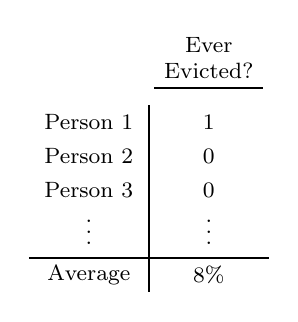
\begin{tikzpicture}[x = .6in, y = .17in, every node/.style={anchor = center, font = \footnotesize}]
\node at (0,-1) {Person 1};
\node at (0,-2) {Person 2};
\node at (0,-3) {Person 3};
\node at (0,-4) {$\vdots$};
\node[anchor = south, align = center] (ev) at (1,0) {Ever\\Evicted?};
\draw[thick] (ev.south west) -- (ev.south east);
\node at (1,-1) {1};
\node at (1,-2) {0};
\node at (1,-3) {0};
\node at (1,-4) {$\vdots$};
\draw[thick] (.5,-.5) -- (.5,-6);
\draw[thick] (-.5,-5) -- (1.5,-5);
\node at (0,-5.5) {Average};
\node at (1,-5.5) {8\%};
\end{tikzpicture}
};
\node<6->[anchor = south] at (bound.north) {\bgray{Lower Bound}};
% Begin the table with predicted
\node<7->[anchor = north east] (predicted) at (16,.9) {
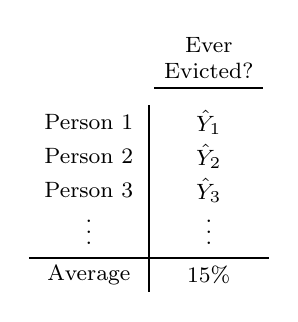
\begin{tikzpicture}[x = .6in, y = .17in, every node/.style={anchor = center, font = \footnotesize}]
\node at (0,-1) {Person 1};
\node at (0,-2) {Person 2};
\node at (0,-3) {Person 3};
\node at (0,-4) {$\vdots$};
\node[anchor = south, align = center] (ev) at (1,0) {Ever\\Evicted?};
\draw[thick] (ev.south west) -- (ev.south east);
\node at (1,-1) {$\hat{Y}_1$};
\node at (1,-2) {$\hat{Y}_2$};
\node at (1,-3) {$\hat{Y}_3$};
\node at (1,-4) {$\vdots$};
\draw[thick] (.5,-.5) -- (.5,-6);
\draw[thick] (-.5,-5) -- (1.5,-5);
\node<8-> at (0,-5.5) {Average};
\node<8-> at (1,-5.5) {15\%};
\end{tikzpicture}
};
\node<7->[anchor = south] at (predicted.north) {\bgray{Predicted Data}};
%\node<7> at (7.5,.5) {\includegraphics[width = \textwidth]{figures/RaceIncomeGroups_largeFont}};
\end{tikzpicture}
\end{frame}

% BEGIN CAUSAL CLAIMS

\roadmap{blue}{0}{.557}{.04}{.557}
\section{Prediction for Causal Claims.}
\roadmap{blue}{0}{.477}{.04}{.477}

% BEGIN JPAM PAPER
\begin{frame}
\centering
\includegraphics[width = .8\textwidth, trim = 0 7.6in 0 1in, clip]{figures/assistance_p1} \vskip .5cm
\begin{footnotesize}Journal of Policy Analysis and Management\\2021\end{footnotesize}
\end{frame}

\begin{frame}
\begin{tikzpicture}[x = \textwidth, y = .9\textheight]
\node at (0,0)  {};
\node at (1,1) {};
% BEGIN TIMELINE AT BOTTOM
\node[anchor = south] at (.5,0) {
\begin{tikzpicture}[x = \textwidth / 17, y = .5\textheight, every node/.style={anchor = center}]
\draw[thick] (-1,.1) -- (16,.1);
\foreach \i in {0, 1,3,5,9,15} {
\draw[thick] (\i,.09) -- (\i,.11);
\node[font = \footnotesize, anchor = north] at (\i,.09) {\i};
}
\node[font = \footnotesize] at (7.5,0) {Child Age};
% Note the age 9-15 report
\draw[thick] (9,.2) -- (15,.2);
\node[anchor = north, font = \scriptsize, gray] (t_label) at (9,.38) {Treatment};
\draw[->, thick, gray] (t_label) -- (9,.22); 
\draw[thick, gray] (0,.28) -- (8.8,.27);
\node[font = \scriptsize, gray, fill = white] at (4.5,.27) {Covariates};
\node[font = \scriptsize, gray, fill = white] at (12,.27) {Outcome};
\node[font = \footnotesize] at (15,.2) {$\bullet$};
\node[anchor = north, font = \footnotesize] at (12,.2) {Were you evicted?};
%\node[font = \footnotesize, align  = center] (difficult) at (12,.4) {Very difficult\\to predict\\for individuals};
%\draw[->, thick] (difficult) -- (12,.25);
% Note the earlier reports
\foreach \i in {1,3,5,9} {
\draw[thick] (\i - 1,.2) -- (\i,.2);
\node[font = \footnotesize] at (\i,.2) {$\bullet$};
}
\end{tikzpicture}};
% END TIMELINE
%\node[anchor = north west] at (0,1) {Prediction for causal claims};
%\node[anchor = north west, font = \small] at (0,.95) {Outcome variable $Y$: Eviction};
%\node[anchor = north west, font = \large] at (0,.95) {Estimation via outcome modeling};
% Factual science table is its own tikzppicture
\node[anchor = north west] (factual) at (0,.9) {
\scalebox{.7}{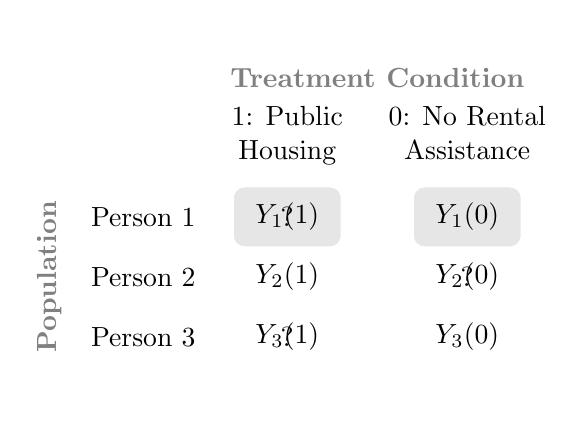
\begin{tikzpicture}[x = .9in, y = .3in, every node/.style={anchor = center}]
\node at (0,-4) {};
\node at (0,2) {};
\node[anchor = south, align = center, font = \bf, gray, rotate = 90] at (-.2,-2) {Population};
\node at (.2,-1) {Person 1};
\node at (.2,-2) {Person 2};
\node at (.2,-3) {Person 3};
\node[anchor = south, align = center, font = \bf, gray] at (1.5,1) {Treatment Condition};
\node[anchor = north, align = center] at (1,1) {1: Public\\Housing};
\node[anchor = north, align = center] at (2,1) {0: No Rental\\Assistance};
\draw<3,5>[color = white, fill = gray, fill opacity = .2, rounded corners] (.7,-1.5) rectangle (1.3,-.5);
\draw<4-5>[color = white, fill = gray, fill opacity = .2, rounded corners] (1.7,-1.5) rectangle (2.3,-.5);
\node<2-5> at (1,-1) {$Y_1(1)$};
\node<2-> at (2,-1) {$Y_1(0)$};
\node<2-> at (1,-2) {$Y_2(1)$};
\node<2-5> at (2,-2) {$Y_2(0)$};
\node<2-5> at (1,-3) {$Y_3(1)$};
\node<2-> at (2,-3) {$Y_3(0)$};
\node<6-> at (1,-1) {?};
\node<6-> at (2,-2) {?};
\node<6-> at (1,-3) {?};
\end{tikzpicture}}
};
% End factual science table
\node<7->[anchor = south, font = \small] (factual_label) at (factual.north) {Learn a prediction function};
\draw<7->[gray, line width = 1.2pt, line cap = round] (factual_label.south west) -- (factual_label.south east);
% Predicted science table is its own tikzppicture
\node<8->[anchor = north east] (predicted) at (1,.9) {
\scalebox{.7}{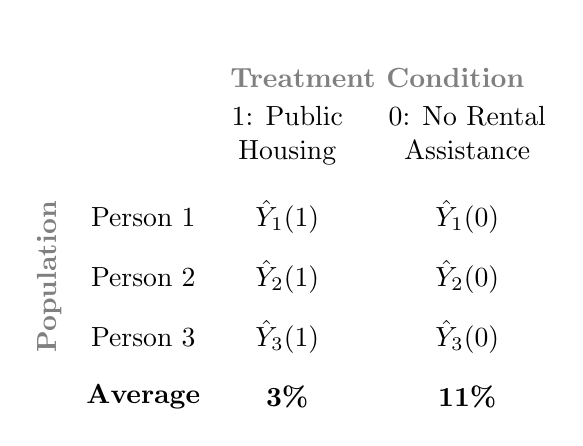
\begin{tikzpicture}[x = .9in, y = .3in, every node/.style={anchor = center}]
\node at (0,-4) {};
\node at (0,2) {};
\node[anchor = south, align = center, font = \bf, gray, rotate = 90] at (-.2,-2) {Population};
\node at (.2,-1) {Person 1};
\node at (.2,-2) {Person 2};
\node at (.2,-3) {Person 3};
\node[anchor = south, align = center, font = \bf, gray] at (1.5,1) {Treatment Condition};
\node[anchor = north, align = center] at (1,1) {1: Public\\Housing};
\node[anchor = north, align = center] at (2,1) {0: No Rental\\Assistance};
\node at (1,-1) {$\hat{Y}_1(1)$};
\node at (2,-1) {$\hat{Y}_1(0)$};
\node at (1,-2) {$\hat{Y}_2(1)$};
\node at (2,-2) {$\hat{Y}_2(0)$};
\node at (1,-3) {$\hat{Y}_3(1)$};
\node at (2,-3) {$\hat{Y}_3(0)$};
%\draw[thick] (.65,-.5) -- (.65,-3.5);
%\draw[thick] (.65,-.5) -- (2.4,-.5);
% Averages that appear on last slides
%\draw<13->[thick] (-.1,-3.5) -- (2.4,-3.5);
\node<13->[font = \bf] at (.2,-4) {Average};
%\draw<13>[thick] (.65,-3.5) -- (.65,-4.5);
\node<13->[font = \bf] at (1,-4) {3\%};
\node<14->[font = \bf] at (2,-4) {11\%};
\end{tikzpicture}}
};
% End predicted science table
\node<8->[anchor = south, font = \small] (predicted_label) at (predicted.north) {Predict the whole table};
\draw<8->[gray, line width = 1.2pt, line cap = round] (predicted_label.south west) -- (predicted_label.south east);
\node<8>[gray, font = \footnotesize, align  = right, anchor = south east] at (1,.4) {Robins 1986\\Hahn 1998};
% Begin DAG
\node<9->[font = \scriptsize, align = center] (x) at (.1,.37) {Measured\\Confounders};
\node<9->[font = \footnotesize] (t) at (.3,.37) {Treatment};
\node<9->[font = \scriptsize] (y) at (.5,.37) {Outcome};
\draw<9->[->, thick] (x) -- (t);
\draw<9->[->, thick] (x) to[bend right] (y);
\draw<9->[->, thick] (t) -- (y);
\node<10>[font = \scriptsize, red] (u) at (.3,.47) {$U$};
\draw<10>[->, thick, dashed, red] (u) -- (t);
\draw<10>[->, thick, dashed, red] (u) -- (y);
%\node<11>[font = \footnotesize, seagreen4] (u) at (.3,.35) {$U$};
%\draw<11>[->, thick, dashed, seagreen4] (u) -- (x);
%\draw<11>[->, thick, dashed, seagreen4] (u) -- (y);
\node<11>[font = \scriptsize, seagreen4] (u) at (.5,.47) {$U$};
\draw<11>[->, thick, dashed, seagreen4] (u) -- (y);
\node<12->[font = \scriptsize, align = center, gray] (this_pop) at (.5,.5) {Those\\factually in\\public housing};
\draw<12->[->, thick, gray] (this_pop) to[bend left] (.55,.6);
%\draw<12->[thick] (-.3,-4) -- (2.5,-4);
%\node<12->[anchor = west] (among) at (.2,.3) {Among those residing in public housing};
%\draw<12->[line width = 1.2pt, gray, line cap = rounded] (among.south west) -- (among.south east);
%\node<12->[anchor = west, blue, font = {\large\bf}] at (.2,.21) {3\%};
%\node<12->[anchor = west] at (.3,.21) {evicted};
%\node<12->[anchor = west, blue, font = {\large\bf}] at (.2,.14) {11\%};
%\node<12->[anchor = west] at (.3,.14) {would have been evicted without help};
\end{tikzpicture}
\end{frame}
% END JPAM PAPER

\begin{frame}
\begin{tikzpicture}[x = \textwidth, y = \textheight]
\node at (0,0)  {};
\node at (1,1) {};
\node at (.25,.7) {That was an old question};
\node[font = \footnotesize] at (.75,.7) {(average treatment effect)};
\node at (.25,.65) {cast in a new way};
\node[font = \footnotesize] at (.75,.65) {(as a prediction task)};
%\node[anchor = west] at (0,.7) {That was an old question};
%\node[anchor = west, font = \footnotesize] at (.5,.7) {(average treatment effect)};
%\node[anchor = west] at (0,.63) {cast in a new way};
%\node[anchor = west, font = \footnotesize] at (.5,.63) {(as a prediction task)};
\node<2->[align = center] at (.5,.4) {Translating to a prediction task also unlocks\\\bblue{new causal questions}};
\node<3>[anchor = north west, font = \small, gray, align = left] at (0,.95) {\textbf{The Gap-Closing Estimand}\\A Causal Approach to Study Interventions\\That Close Disparities Across Social Categories};
\end{tikzpicture}
\end{frame}

% NEW RACE FRAME
\begin{frame}
\begin{tikzpicture}[x = \textwidth, y = \textheight]
\node at (0,0)  {};
\node at (1,1) {};
\node<1-8>[anchor = west] at (0,.8) {The \bblue{causal effect of race} is deeply fraught};
\node<2-6>[rotate = 0] at (.5,.5) {\includegraphics[width = .8\textwidth]{figures/holland_p1}};
\node<3-6>[rotate = 10] at (.5,.5) {\includegraphics[width = .95\textwidth]{figures/greinerrubin_p1}};
\node<4-6>[rotate = 0] at (.5,.5) {\includegraphics[width = .6\textwidth]{figures/senwasow_p1}};
\node<5-6>[rotate = -10] at (.5,.5) {\includegraphics[width = .8\textwidth]{figures/bertrandmullainathan_p1}};
\node<6>[rotate = 5] at (.5,.5) {\includegraphics[width = .8\textwidth]{figures/kohlerhausmann_p1}};
% Begin science table
\node<7>[anchor = north west] at (.05,.77) {
\scalebox{.7}{\begin{tikzpicture}[x = .9in, y = .3in, every node/.style={anchor = center}]
\node at (-1,-4) {};
\node at (0,2) {};
\node[anchor = south, align = center, font = \bf, gray, rotate = 90] at (-.5,-3.5) {Population};
\node at (0,-1) {Person 1};
\node at (0,-2) {Person 2};
\node at (0,-3) {Person 3};
\node at (0,-4) {Person 4};
\node at (0,-5) {Person 5};
\node at (0,-6) {Person 6};
\node[font = \bf, gray] at (1.5,1) {Treatment Condition};
\node at (1,0) {Black};
\node at (2,0) {White};
\draw[thick] (.6,-.5) -- (1.4,-.5);
\draw[thick] (1.6,-.5) -- (2.4,-.5);
\node at (1,-1) {$Y_1(\text{Black})$};
\node at (2,-1) {$Y_1(\text{White})$};
\node at (1,-2) {$Y_2(\text{Black})$};
\node at (2,-2) {$Y_2(\text{White})$};
\node at (1,-3) {$Y_3(\text{Black})$};
\node at (2,-3) {$Y_3(\text{White})$};
\node at (1,-4) {$Y_4(\text{Black})$};
\node at (2,-4) {$Y_4(\text{White})$};
\node at (1,-5) {$Y_5(\text{Black})$};
\node at (2,-5) {$Y_5(\text{White})$};
\node at (1,-6) {$Y_6(\text{Black})$};
\node at (2,-6) {$Y_6(\text{White})$};
\end{tikzpicture}}
};
\node<8->[anchor = north west] at (.05,.77) {
\scalebox{.7}{\begin{tikzpicture}[x = .9in, y = .3in, every node/.style={anchor = center}]
\node at (-1,-4) {};
\node at (0,2) {};
\node<8-15>[anchor = south, align = center, font = \bf, gray, rotate = 90] at (-.5,-2) {Black};
\node<8-15>[anchor = south, align = center, font = \bf, gray, rotate = 90] at (-.5,-5.5) {White};
\node<16>[anchor = south, align = center, font = \bf, gray, rotate = 90] at (-.5,-2) {Category A};
\node<16>[anchor = south, align = center, font = \bf, gray, rotate = 90] at (-.5,-5.5) {Category B};
\draw[line width = 1.2pt, gray] (-.45,-.7) -- (-.45,-3.3);
\draw[line width = 1.2pt, gray] (-.45,-4.2) -- (-.45,-6.8);
\node at (0,-1) {Person 1};
\node at (0,-2) {Person 2};
\node at (0,-3) {Person 3};
\node at (0,-4.5) {Person 4};
\node at (0,-5.5) {Person 5};
\node at (0,-6.5) {Person 6};
%\node[font = \bf, gray] at (1.5,1) {Treatment Condition};
\only<11->{
\draw[draw = white, fill = gray, fill opacity = .2, rounded corners] (.7,-3.5) rectangle (1.3, -.5);
\draw[draw = white, fill = gray, fill opacity = .2, rounded corners] (.7,-7) rectangle (1.3, -4);
\node[anchor = north, font = \bf, gray, align = center] at (1,-7.3) {Descriptive\\Disparity};
}
\only<13->{
\draw[draw = white, fill = gray, fill opacity = .2, rounded corners] (1.7,-3.5) rectangle (2.3, -.5);
\draw[draw = white, fill = gray, fill opacity = .2, rounded corners] (1.7,-7) rectangle (2.3, -4);
\node[anchor = north, font = \bf, gray, align = center] at (2,-7.3) {Gap-Closing\\Estimand};
}
\only<10->{
\node[align = center] at (1,.4) {As\\observed};
\draw[thick] (.6,-.3) -- (1.4,-.3);
\node at (1,-1) {$Y_1$};
\node at (1,-2) {$Y_2$};
\node at (1,-3) {$Y_3$};
\node at (1,-4.5) {$Y_4$};
\node at (1,-5.5) {$Y_5$};
\node at (1,-6.5) {$Y_6$};
}
\only<12->{
\node[align = center] at (2,.4) {Under\\intervention};
\draw[thick] (1.6,-.3) -- (2.4,-.3);
\node at (2,-1) {$Y_1(t)$};
\node at (2,-2) {$Y_2(t)$};
\node at (2,-3) {$Y_3(t)$};
\node at (2,-4.5) {$Y_4(t)$};
\node at (2,-5.5) {$Y_5(t)$};
\node at (2,-6.5) {$Y_6(t)$};
}
\end{tikzpicture}}
};
\node<14->[anchor = west] at (0,.8) {Can an intervention \bblue{close the gap}?};
\node<15->[anchor = east, font = \footnotesize, align = right, gray] at (1,.3) {Vanderweele \&\\Robinson 2014\\{}\\Jackson \&\\Vanderweele 2018};
\end{tikzpicture}
\end{frame}

% CHETTY
% Other examples
\begin{frame}
\begin{tikzpicture}[x = \textwidth, y = \textheight]
\node at (0,0) {};
\node at (1,1) {};
%%%%%%%%%%%
% CHETTY  ET AL %
%%%%%%%%%%%
\node<1-3> at (.5,.5) {\includegraphics[width = \textwidth]{figures/chetty_figure_1}};
\node<4> at (.5,.5) {\includegraphics[width = \textwidth]{figures/chetty_figure_2}};
\node<5-> at (.5,.5) {\includegraphics[width = \textwidth]{figures/chetty_figure_3}};
\node<1->[anchor = south east, font = {\footnotesize\bf}, color = gray] at (1,.1) {Chetty et al. 2017};
\node<2-3>[anchor = north, font = \small] at (.5,.46) {The average child lands at the};
\node<2-3>[anchor = north west, align = left, font = \scriptsize] at (.1, .4) {\bblue{34th percentile} of income\\if their parents were at\\the \bblue{bottom} of the distribution};
\draw<2-3>[->, thick, blue] (.15,.4) to[bend left] (.15,.44);
\node<3>[anchor = north east, align = right, font = \scriptsize] at (.85, .4) {\bblue{65th percentile} of income\\if their parents were at\\the \bblue{top} of the distribution};
\draw<3>[->, thick, blue] (.83,.4) to[out = 90, in = 350] (.8,.6) to[out = 170, in = 0] (.77, .6);
\draw<6->[->, thick, seagreen4] (.173,.5) -- (.173, .61);
\draw<6->[->, thick, seagreen4] (.751,.62) -- (.751, .64);
\end{tikzpicture}
\end{frame}

\begin{frame}
\begin{tikzpicture}[x = \textwidth, y = .9\textheight]
\node at (0,0) {};
\node at (1,1) {};
\node[anchor = north west] at (0,.95) {Define the research goal by a \bgray{target trial} \begin{scriptsize}(Hern\'an \& Robins 2016)\end{scriptsize}};
\node<6->[anchor = north west] (local) at (0,.65) {Local intervention};
\node<2->[anchor = north west, font = \footnotesize] at (0,.55) {1.};
\node<3->[anchor = north west, font = \footnotesize] at (0,.5) {2.};
\node<4->[anchor = north west, font = \footnotesize, align = left] at (0,.45) {3.};
\node<2->[anchor = north west, font = \footnotesize] at (.03,.55) {Sample $\mathcal{S}$ from the population};
\node<3->[anchor = north west, font = \footnotesize] at (.03,.5) {Assign treatment $T = 1$ to $\mathcal{S}$};
\node<4->[anchor = north west, font = \footnotesize, align = left] at (.03,.45) {Observe the disparity\\across categories $X$};
\node<5->[anchor = north west, font = \footnotesize, align = left] at (0,.3) {Goal: };
\node<5->[anchor = north west, font = \footnotesize, align = left] at (.1,.3) {Expected result over\\hypothetical samples $\mathcal{S}$};
\node<12->[anchor = north west, font = \footnotesize, align = left] at (0,.15) {Difficulty:};
\node<12->[anchor = north west, font = \footnotesize, align = left] at (.15,.15) {Causal inference};
%%%%%%%
\node<7->[anchor = north west] (global) at (.55,.65) {Global intervention};
\node<8->[anchor = north west, font = \footnotesize] at (.55,.55) {1.};
\node<9->[anchor = north west, font = \footnotesize] at (.55,.5) {2.};
\node<10->[anchor = north west, font = \footnotesize, align = left] at (.55,.45) {3.};
\node<8->[anchor = north west, font = \footnotesize] at (.58,.55) {Take the entire population $\mathcal{P}$};
\node<9->[anchor = north west, font = \footnotesize] at (.58,.5) {Assign treatment $T = 1$ to $\mathcal{P}$};
\node<10->[anchor = north west, font = \footnotesize, align = left] at (.58,.45) {Observe the disparity\\across categories $X$};
\node<11->[anchor = north west, font = \footnotesize, align = left] at (.55,.3) {Goal: };
\node<11->[anchor = north west, font = \footnotesize, align = left] at (.65,.3) {Result of this procedure};
\node<12->[anchor = north west, font = \footnotesize, align = left] at (.55,.15) {Difficulty:};
\node<12->[anchor = north west, font = \footnotesize, align = left] (diff2a) at (.7,.15) {Causal inference};
\node<13->[anchor = north west, font = \footnotesize, align = left] at (diff2a.south west) {Equilibrium dynamics};
% Tension
\draw<14->[line width = 2.5pt] (.25,.7) -- (.75, .7);
\node<14->[font = \Huge] at (.25,.7) {$\bullet$};
\node<14->[font = \Huge] at (.75,.7) {$\bullet$};
\node<15>[anchor = south, align = right, font = \footnotesize, gray] at (.7,.77) {Policy-relevant?};
\draw<15>[->, thick, gray] (.7,.77) -- (.7,.72);
\node<16>[anchor = south, align = right, font = \footnotesize, gray] at (.3,.77) {Policy-relevant.};
\draw<16>[->, thick, gray] (.3,.77) -- (.3,.72);
\end{tikzpicture}
\end{frame}

\roadmap{blue}{.05}{.397}{.09}{.397}
\roadmap{blue}{.05}{.347}{.09}{.347}

\begin{frame}
\label{dag}
\begin{tikzpicture}[x = \textwidth, y = \textheight]
\node at (-.05,0) {};
\node at (.9,1) {};
%\node[anchor = north west, align = left] at (.25,.95) {We have to impute the outcome each person $i$\\would realize in each occupation $t$};
\node<1->[anchor = east, align = left, font = \small, gray] at (.9,.1) {Pearl 2009};%Hern\'an \& Robins 2020};
\node<2,5->[align = center] (l) at (.2,.45) {Measured\\Confounders};
\node<3-4>[draw, rounded corners, align = center] (l) at (.2,.45) {Measured\\Confounders};
\node<1-2,5->[align = center] (x) at (.2,.75) {Gap-Defining\\Category};
\node<3-4>[draw, rounded corners, align = center] (x) at (.2,.75) {Gap-Defining\\Category};
\node<1-> (t) at (.5,.6) {Treatment};
\node<1-> (y) at (.8,.6) {Outcome};
\node<1->[font = \scriptsize, gray, align = center, anchor = east] at (x.west) {parent\\income};
\node<1->[font = \scriptsize, gray, align = center, anchor = north] at (t.south) {selective\\college};
\node<1->[font = \scriptsize, gray, align = center, anchor = north] (y_label) at (y.south) {respondent\\income};
\node<2->[font = \scriptsize, gray, align = left, anchor = north] (l_label) at (l.south) {SAT score\\High school GPA\\Colleges applied};
\draw<2->[->, thick] (l) -- (t.south west);
\draw<2->[->, thick] (l) to[bend right = 15] (y.south west);
\draw<1->[->, line width = 2pt, blue] (t) -- (y);
\draw<1->[->, thick] (x) -- (t.north west);
\draw<2->[->, thick] (x) -- (l);
\draw<1->[->, thick] (x) to[bend left = 40] (y);
% Confounding of X is ok
\node<5->[align = center] (v) at (.05,.13) {Unobserved\\Things};
\draw<5->[->, thick, dashed] (v) to[bend left = 20] (x);
\draw<5->[->, thick, dashed] (v) -- (l_label);
\draw<5->[->, thick, dashed] (v) to[out = 0, in = 240] (y_label); 
% Confounding of T is bad
\node<4>[red] (u) at (.5,.7) {$U$};
\draw<4>[->, red, line width = 2pt] (u) -- (t);
\draw<4>[->, red, line width = 2pt] (u) -- (y); 
\end{tikzpicture}
\end{frame}

\roadmap{blue}{.05}{.347}{.09}{.347}
\roadmap{blue}{.05}{.297}{.09}{.297}

\begin{frame}
\begin{tikzpicture}[x = \textwidth, y = .9\textheight]
\node at (0,0)  {};
\node at (1,1) {};
%\node<3->[anchor = north] (solution) at (.5,.95) {Solution: Reweight errors to approximate the correct task};
%\draw<3->[gray, line width = 1.2pt, line cap = round] (solution.south west) -- (solution.south east);
\node<6->[anchor = north west, font = \small] at (0,.9) {Estimated bias:};
\node<6->[align = left, anchor = north west, font = \small] at (.25,.91) {Mean($\hat{Y}_i - Y_i$) with\\inverse probability of treatment weights};
% Table illustrating IPTW
\node<2-7>[anchor = north west] (factual) at (.1,.65) {
\scalebox{.7}{\begin{tikzpicture}[x = .8in, y = .3in, every node/.style={anchor = center}]
\node at (0,-4) {};
\node at (0,2) {};
\node at (0,-1) {Person 1};
\node at (0,-2) {Person 2};
\node at (0,-3) {Person 3};
\node at (0,-4.5) {Person 4};
\node at (0,-5.5) {Person 5};
\node at (0,-6.5) {Person 6};
\node[font = \bf, gray, align = center] at (-1.2,-2) {People in\\category 1};
\node[font = \bf, gray, align = center] at (-1.2,-5.5) {People in\\category 2};
\draw[line cap = round, gray, line width = 2pt] (-.5,-.6) -- (-.5,-3.4);
\draw[line cap = round, gray, line width = 2pt] (-.5,-4.1) -- (-.5,-6.9);
\node[anchor = south, align = center] at (1,0) {Prediction\\under\\treatment};
\node at (1,-1) {$\hat{Y}_1(1)$};
\node at (1,-2) {$\hat{Y}_2(1)$};
\node at (1,-3) {$\hat{Y}_3(1)$};
\node at (1,-4.5) {$\hat{Y}_4(1)$};
\node at (1,-5.5) {$\hat{Y}_5(1)$};
\node at (1,-6.5) {$\hat{Y}_6(1)$};
\node<3->[anchor = south, align = center] at (2,0) {Outcome\\under\\treatment};
\node<3-> at (2,-1) {?};
\node<3-> at (2,-2) {$Y_2$};
\node<3-> at (2,-3) {$Y_3$};
\node<3-> at (2,-4.5) {?};
\node<3-> at (2,-5.5) {$Y_5$};
\node<3-> at (2,-6.5) {?};
\node<4->[anchor = south, align = center] at (3,0) {Error};
\node<4-> at (3,-1) {?};
\node<4-> at (3,-2) {$\hat{Y}_2(1) - Y_2$};
\node<4-> at (3,-3) {$\hat{Y}_3(1) - Y_3$};
\node<4-> at (3,-4.5) {?};
\node<4-> at (3,-5.5) {$\hat{Y}_5(1) - Y_5$};
\node<4-> at (3,-6.5) {?};
\node<5->[anchor = south, align = center] at (4,0) {Weight\\on error};
\node<5-> at (4,-2) {3 / 2};
\node<5-> at (4,-3) {3 / 2};
\node<5-> at (4,-5.5) {$3$};
\draw[color = white, fill = gray, opacity = .2, rounded corners] (.5,-3.5) rectangle (1.5,-.5);
\draw[color = white, fill = gray, opacity = .2, rounded corners] (.5,-7) rectangle (1.5,-4);
\end{tikzpicture}}
};
% End table illustrating IPTW
% Begin doubly robust
\node<7->[anchor = north west, align = center, font = \small] at (0,.75) {New Estimate:};
\node<7->[anchor = north west, font = \small] at (.25,.75) {(Original Estimate) $-$ (Estimated Bias)};
\node<7->[anchor = north east, font = \footnotesize, align = right, gray] at (1,.75) {Doubly\\Robust\\Estimation};
\node<7-12>[anchor = south east, font = \footnotesize, align = right, gray] at (1,0) {Robins, Rotnitzky, \& Zhao 1994\\Bang \& Robins 2005};
\node<8>[anchor = north] at (.5,.5) {\includegraphics[width = \textwidth]{figures/sim_x1mx0_0}};
\node<9>[anchor = north] at (.5,.5) {\includegraphics[width = \textwidth]{figures/sim_x1mx0_1}};
\node<10>[anchor = north] at (.5,.5) {\includegraphics[width = \textwidth]{figures/sim_x1mx0_2}};
\node<11>[anchor = north] at (.5,.5) {\includegraphics[width = \textwidth]{figures/sim_x1mx0_3}};
% Begin DML
\node<12->[anchor = north west, font = \small] at (0,.55) {Even better:};
\node<12->[anchor = north east, font = \footnotesize, align = right, gray] at (1,.55) {Double\\Machine\\Learning};
\node<13->[anchor = north west, font = \small] (sample_split_A) at (.25,.56) {--- Learn $\hat{Y}_i$ in sample A};
\node<14->[anchor = north west, font = \small] (sample_split_B) at (sample_split_A.south west) {--- Estimate bias in sample B};
\node<15->[anchor = north west, font = \small] (sample_split_C) at (sample_split_B.south west) {--- Cross fit: Swap roles and average};
\node<16> at (.5,.5) {\includegraphics[width = \textwidth]{figures/sim_cross_fitting_convergence_1}};
\node<17-18> at (.5,.5) {\includegraphics[width = \textwidth]{figures/sim_cross_fitting_two}};
\draw<16>[draw = white, fill = white] (.7,.32) rectangle (1,.63);
\draw<16-18>[draw = white, fill = white] (.7,.42) rectangle (1,.63);
%\node<18> at (.5,.5) {\includegraphics[width = \textwidth]{figures/sim_cross_fitting_convergence_3}};
%\node<19> at (.5,.5) {\includegraphics[width = \textwidth]{figures/sim_cross_fitting_convergence_4}};
%\node<18->[anchor = north east, font = \footnotesize, align = right] at (1,.25) {Double\\Machine\\Learning};
\node<13-15>[anchor = south east, font = \footnotesize, align = right, gray] at (1,0) {Chernozhukov et al. 2018\\Bickel 1982};
\node<18->[red, draw, fill = white, rounded corners, line width = 2pt, font = {\footnotesize\bf}, rotate = 20] at (.6,.8) {So complicated!};
\end{tikzpicture}
\end{frame}

\begin{frame}[t,fragile]
\includegraphics[width = .9\textwidth]{figures/gapclosing_cran}
Available from CRAN: \texttt{install.packages("gapclosing")} \\ \pause
\begin{scriptsize}
\begin{verbatim}
estimate <- gapclosing(
  data = simulated_data,
  outcome_formula = formula(outcome ~ category + confounder),
  treatment_formula = formula(treatment ~ category + confounder),
  category_name = "category",
  counterfactual_assignments = 1,
  outcome_algorithm = "ranger",
  treatment_algorithm = "ranger",
  sample_split = "cross_fit",
  se = T
)
\end{verbatim} \pause

\begin{verbatim}
Counterfactual mean outcomes (post-intervention means):
   category estimate     se ci.min ci.max
   <chr>       <dbl>  <dbl>  <dbl>  <dbl>
 1 A         -0.102  0.154  -0.404  0.200
 2 B          0.0409 0.0978 -0.151  0.233
 \end{verbatim}
 \end{scriptsize}
\end{frame}

\roadmap{blue}{.05}{.297}{.09}{.297}
\roadmap{blue}{.05}{.247}{.09}{.247}

% EXAMPLE 1: ECONOMIC MOBILITY
\begin{frame}
\begin{tikzpicture}[x = \textwidth, y = \textheight]
\node at (0,0) {};
\node at (1,1) {};
\node[anchor = west] at (0,.95) {\bblue{Empirical Example 1}: Economic Mobility};
% DAG
\onslide<1-4>{
\node (x) at (.2,.6) {$X$};
\node[anchor = east, font = \footnotesize, align = center] (x_label) at (x.west) {Father's\\Social Class};
\node[anchor = north, font = \scriptsize, align = center, gray] at (x_label.south) {Professional\\or\\Working Class};
\node (y) at (.8,.6) {$Y$};
\node[font = \footnotesize, align = center, anchor = west] at (y.east) {Your\\Income};
\draw[<->, thick] (x) to[out = 90, in = 90] (y);
}
\onslide<2-4>{
\node[anchor = south, font = \footnotesize, align = center] at (t.north) {Your\\Social Class};
\node (t) at (.5,.6) {$T$};
\draw<2-3>[->, thick] (x) -- (t);
\draw[->, thick] (t) -- (y);
}
\onslide<3-4>{
\node (l) at (.2,.4) {$\vec{L}$};
\draw[<->, thick] (x) -- (l);
\draw<3>[->, thick] (l) -- (t);
\draw[->, thick] (l) to[bend right = 15] (y);
\node[anchor = north, font = \footnotesize, align = left] at (l.south) {Race, Sex,\\Age, Education};
}
\onslide<4>{
\node[font = {\scriptsize\bf}, blue]  (intervention) at (.35,.5) {Intervention};
\draw[->, thick, snake = zigzag, blue, line before snake = 10pt, line after snake = 10pt, segment length = 4pt] (intervention) -- (t);%(.43,.52) -- (.48,.58);
}
% Result
\node<5>[anchor = south] at (.5,.1) {\includegraphics[width = \textwidth]{figures/empirical_example_slide_0}};
\node<6>[anchor = south] at (.5,.1) {\includegraphics[width = \textwidth]{figures/empirical_example_slide_1}};
\node<7>[anchor = south] at (.5,.1) {\includegraphics[width = \textwidth]{figures/empirical_example_slide_2}};
\node<8>[anchor = south] at (.5,.1) {\includegraphics[width = \textwidth]{figures/empirical_example_slide_3}};
%\node<9>[anchor = east, draw, rounded corners] at (.97,.87) {\texttt{plot\_two\_categories()}};
\end{tikzpicture}
\end{frame}

% EXAMPLE 2: OCCUPATIONAL SEGREGATION
\begin{frame}
\begin{tikzpicture}[x = \textwidth, y = \textheight]
\node at (0,0) {};
\node at (1,1) {};
\node[anchor = west] at (0,.95) {\bblue{Empirical Example 2}: Racial Disparities in Health};
% DAG
\onslide<1-4>{
\node (x) at (.2,.6) {$X$};
\node[anchor = east, font = \footnotesize, align = center] (x_label) at (x.west) {Race};
\node (y) at (.8,.6) {$Y$};
\node[font = \footnotesize, align = center, anchor = west] at (y.east) {Onset of\\work-limiting\\disability};
\draw[<->, thick] (x) to[out = 90, in = 90] (y);
}
\onslide<2-4>{
\node[anchor = south, font = \footnotesize, align = center] at (t.north) {Occupation};
\node (t) at (.5,.6) {$T$};
\draw<2-3>[->, thick] (x) -- (t);
\draw[->, thick] (t) -- (y);
}
\onslide<3-4>{
\node (l) at (.2,.4) {$\vec{L}$};
\draw[<->, thick] (x) -- (l);
\draw<3>[->, thick] (l) -- (t);
\draw[->, thick] (l) to[bend right = 15] (y);
\node[anchor = north, font = \footnotesize, align = left] at (l.south) {Sex,\\Age, Education\\Foreign born,\\Lagged outcome,\\Lagged health};
}
\onslide<4>{
\node[font = {\scriptsize\bf}, blue]  (intervention) at (.35,.5) {Intervention};
\draw[->, thick, snake = zigzag, blue, line before snake = 10pt, line after snake = 10pt, segment length = 4pt] (intervention) -- (t);
}
% Result
\node<5>[anchor = south] at (.5,.1) {\includegraphics[width = \textwidth]{figures/segregation_slide_0}};
\node<6>[anchor = south] at (.5,.1) {\includegraphics[width = \textwidth]{figures/segregation_slide_1}};
\node<7>[anchor = south] at (.5,.1) {\includegraphics[width = \textwidth]{figures/segregation_slide_2}};
\node<8>[anchor = south] at (.5,.1) {\includegraphics[width = \textwidth]{figures/segregation_slide_3}};
\end{tikzpicture}
\end{frame}

\begin{frame}
\begin{tikzpicture}[x = \textwidth, y = \textheight]
\node at (0,0) {};
\node at (1,1) {};
\node[anchor = west, font = \large] at (0,.85) {\bblue{Future applications}};
\node<1->[anchor = west, align = left] at (0,.7) {The gap-closing estimand can\\help us understand disparities by};
\node<1->[anchor = west, font = \small] at (0,.6) {--- Race};
\node<1->[anchor = west, font = \small] at (0,.55) {--- Class};
\node<1->[anchor = west, font = \small] at (0,.5) {--- Gender};
\node<2->[anchor = west] at (0,.4) {and develop interventions to \bblue{close those gaps}.};
\end{tikzpicture}
\end{frame}

\begin{frame}{\large Contribution to methodology: Bringing perspectives together}%How the gap-closing estimand contributes to methodology}
\begin{tikzpicture}[x = .8\textwidth, y = .12\textheight]
\node[align = left] at (1,0) {\phantom{Gap-Closing Estimand}};
\node<2->[anchor = west, align = left, font = \footnotesize] (s1) at (0,6) {Interventions to Close Disparities\\{\footnotesize Biostatistics: Jackson \& Vanderweele 2018}};
\node<3->[anchor = west, align = left, font = \footnotesize] (s2) at (0,5) {Doubly Robust Estimators\\{\footnotesize Biostatistics: Bang \& Robins 2005}};
\node<4->[anchor = west, align = left, font = \footnotesize] (s3) at (0,4) {Double Machine Learning\\{\footnotesize Econometrics: Chernozhukov et al. 2018}};
\node<5->[anchor = west, align = left, font = \footnotesize] (s4) at (0,3) {Variance Estimation by Balanced Repeated Replicates\\{\footnotesize Survey Methodology: Krewski \& Rao 1981}};
\node<6->[anchor = west, align = left, font = \footnotesize] (s5) at (0,1.85) {Social Construction of Race\\{\footnotesize Sociology: Omi \& Winant 1994}\\{\footnotesize Law: Kohler-Hausmann 2018}};
\node<7->[anchor = west, align = left, font = \footnotesize] (s6) at (0,.72) {Local Interpretation};
\node<8->[align = left] (this) at (1,0) {Gap-Closing Estimand};
\draw<8->[->, thick] (s1) -- (1,6) -- (this);
\draw<8->[->, thick] (s2) -- (1,5) -- (this);
\draw<8->[->, thick] (s3) -- (1,4) -- (this);
\draw<8->[->, thick] (s4) -- (1,3) -- (this);
\draw<8->[->, thick] (s5) -- (1,1.85) -- (this);
\draw<8->[->, thick] (s6) -- (1,.72) -- (this);
\end{tikzpicture}
\end{frame}

\roadmap{blue}{0}{.477}{.04}{.477}
\section{Closing Argument.}
\roadmap{white}{0}{.477}{.04}{.477}

\begin{frame}
\begin{tikzpicture}[x = \textwidth, y = .9\textheight]
\node at (0,0) {};
\node at (1,1) {};
\node[anchor = north west, font = \Large] at (0,1) {\bgray{Prediction in Social Science}};
\node[anchor = north west] at (0, .92) {A Tool to Study Inequality in Populations};
\node[font = \small] (data) at (.25,.75) {Data scientists:};
\node[font = \footnotesize, fill = gray, rounded corners, fill opacity = .2, text opacity = 1] (data_quote) at (.25,.68) {Predict for individuals!};
\node[font = \small] (social) at (.75,.75) {Social scientists:};
\node[font = \footnotesize, fill = gray, rounded corners, fill opacity = .2, text opacity = 1] (social_quote) at (.75,.68) {I don't do prediction.};
% Why data scientists are wrong
\draw<2-3>[rounded corners, thick] (.05,.62) rectangle (.45,.79);
\node<3>[anchor = west] (apple_fig_1) at (0,.4) {\includegraphics[width = .2\textwidth]{figures/20061107apple.jpg}};
\node<3>[anchor = west, font = \small] (apple_lab_1) at (.3,.4) {Apple};
\draw<3>[->, thick] (apple_fig_1) -- (apple_lab_1);
\node<3> (person_fig_1) at (.6,.4) {\includegraphics[width = .04\textwidth]{figures/stickFigure}};
\node<3>[anchor = west, font = \small] (person_lab_1) at (.8,.4) {Evicted};
\draw<3>[->, thick] (person_fig_1) to node[midway, above, font = \footnotesize, align = center] {very\\difficult} (person_lab_1);
% Why social scientists are wrong
\draw<4-11>[rounded corners, thick] (.55,.62) rectangle (.95,.79);
\draw<5-11>[->, thick] (.75,.62) -- (.75,.55);
\node<5-11>[anchor = north west, font = \small] at (.62,.53) {I take [data source]};
\node<5-11>[anchor = north west, font = \small] at (.62,.47) {I estimate $\beta_1$};
\node<5-11>[anchor = north west, font = \small] at (.62,.4) {$Y = \beta_0 + X_1\beta_1$};
\node<5-11>[anchor = north west, font = \small] at (.69,.33) {$+ X_2\beta_2 + \epsilon$};
%\draw<7->[->, thick, gray] (.22, .4) -- (.22, .44);
%\node<7->[anchor = north, align = center, font = \footnotesize, gray] at (.22,.4) {$\beta_1$ is an estimand\\that assumes a model};
\node<6-11>[anchor = north west, align = left, font = \footnotesize, fill = seagreen4, fill opacity = .2, text opacity = 1, rounded corners] at (0,.55) {What if the\\model is wrong?};
\node<7-11>[anchor = north east, align = right, font = \footnotesize, fill = gray, rounded corners, fill opacity = .25, text opacity = 1] at (.55,.47) {The model is an\\approximation};
\node<8-11>[anchor = north west, align = left, font = \footnotesize, fill = seagreen4, rounded corners, fill opacity = .2, text opacity = 1] at (0,.39) {So $\beta_1$ is an\\approximation to...};
\node<9-11>[anchor = north east, align = right, font = \footnotesize, fill = gray, rounded corners, fill opacity = .2, text opacity = 1] at (.55,.31) {Something. I just\\haven't said what.};
\node<10-11>[anchor = north west, align = left, font = \footnotesize, fill = seagreen4, rounded corners, fill opacity = .2, text opacity = 1] at (0,.23) {Is it a good\\approximation?};
\node<11>[anchor = north east, align = right, font = \footnotesize, fill = gray, rounded corners, fill opacity = .2, text opacity = 1] at (.55,.15) {\bred{Epistemological}\\\bred{crisis}};
% Estimands starts on slide 13
\node<13->[align = left, font = \footnotesize, anchor = south west, gray] at (0,0) {Lundberg, Johnson, Stewart\\\textbf{What is Your Estimand?}\\Forthcoming, \emph{American Sociological Review}};
% Begin the proposed estimand statement
\node<14->[circle, fill = lightgray, draw = lightgray, font = \footnotesize, inner sep = 8pt] (point1) at (.65,.5) {};
\node<15>[font = \scriptsize] at (point1) {$Y_i$};
\node<16>[font = \scriptsize] at (point1) {$Y_i(t)$};
\node<14->[gray, font = \footnotesize, align = center, anchor = north] (usqNote) at (point1.south) {A \bgray{unit-specific}\\\bgray{quantity}};
\node<17->[circle, fill = lightgray, draw = lightgray, font = \footnotesize, inner sep = 8pt] (point2) at (.8,.47) {};
\node<17->[circle, fill = lightgray, draw = lightgray, font = \footnotesize, inner sep = 8pt] (point3) at (.7,.28) {};
\node<17->[circle, fill = lightgray, draw = lightgray, font = \footnotesize, inner sep = 8pt] (point4) at (.85,.33) {};
\node<17->[circle, fill = lightgray, draw = lightgray, font = \footnotesize, inner sep = 8pt] (point5) at (.58,.3) {};
\node<17->[circle, fill = lightgray, draw = lightgray, font = \footnotesize, inner sep = 8pt] (point6) at (.9,.5) {};
\draw<17->[line width = 2pt, gray, rounded corners] (.53,.2) rectangle (.97,.57);
\node<17->[gray, font = \footnotesize, align = center, anchor = north] at (.75,.2) {Aggregated over a\\\bgray{target population}};
\node<17->[font = \scriptsize] at (point1) {$Y_1(t)$};
\node<17-18>[font = \scriptsize] at (point2) {$Y_2(t)$};
\node<17->[font = \scriptsize] at (point3) {$Y_5(t)$};
\node<17-18>[font = \scriptsize] at (point4) {$Y_6(t)$};
\node<17-18>[font = \scriptsize] at (point5) {$Y_4(t)$};
\node<17->[font = \scriptsize] at (point6) {$Y_3(t)$};
%\node<18-23>[anchor = north west, align = left] (caption1) at (0,.52) {Our framework expands \bblue{theory},};
%\node<18-23>[anchor = north west, align = left] (caption2) at (caption1.south west) {links to transparent \bblue{evidence},};
%\node<18-23>[anchor = north west, align = left] at (caption2.south west) {and unlocks computational \bblue{tools}};
%\draw<19>[line width = 2pt, blue] (.375,.45) -- (.48,.45);
%\draw<20-21>[line width = 2pt, blue] (.31,.385) -- (.46,.385);
%\draw<22-23>[line width = 2pt, blue] (.425,.32) -- (.503,.32);
\node<18-19>[circle, draw = black, font = \footnotesize, inner sep = 8pt, line width = 1.2pt] at (point1) {};
\node<18-19>[circle, draw = black, font = \footnotesize, inner sep = 8pt, line width = 1.2pt] at (point3) {};
\node<18-19>[circle, draw = black, font = \footnotesize, inner sep = 8pt, line width = 1.2pt] at (point6) {};
\node<19>[font = \scriptsize] at (point2) {$\hat{Y}_2(t)$};
\node<19>[font = \scriptsize] at (point4) {$\hat{Y}_6(t)$};
\node<19>[font = \scriptsize] at (point5) {$\hat{Y}_4(t)$};
% Summary statement
\node<13->[anchor = west, font = \small] at (0,.52) {The \bblue{estimand}};
\node<13->[anchor = west, font = \small] at (0,.47) {connects social science};
\node<13->[anchor = west, font = \small] at (0,.42) {to data science};
\node<13->[anchor = west, font = \small] at (0,.37) {via \bblue{prediction}};
\end{tikzpicture}
\end{frame}

\begin{frame}
\begin{tikzpicture}[x = \textwidth, y = .9\textheight]
\node at (0,0) {};
\node at (1,1) {};
\node[anchor = north west, font = \Large] at (0,1) {\bgray{Prediction in Social Science}};
\node[anchor = north west] at (0, .92) {A Tool to Study Inequality in Populations};
\node[anchor = north west, font = \small] at (0, .75) {Three possible uses:};
\node[anchor = north west, font = \small] at (0.05,.67) {1)};
\node[anchor = north west, font = \small] at (0.05,.59) {2)};
\node[anchor = north west, font = \small] at (0.05,.51) {3)};
\node[anchor = north west, font = \small] at (.1,.67) {Prediction for individuals};
\node[anchor = north west, align = left, font = \small] at (.1,.59) {Prediction for description};
\node[anchor = north west, align = left, font = \small] at (.1,.51) {Prediction for causal claims};
\node[anchor = north east, font = \small] at (1,.67) {very hard};
\node[anchor = north east, font = \small] at (1,.59) {useful};
\node[anchor = north east, font = \small, align = right] at (1,.51) {opportunities\\abound};
\node[anchor = north west, font = \footnotesize, align = left] at (.1, .43) {--- Define the intervention};
\node[anchor = north west, font = \footnotesize, align = left] at (.1, .38) {--- Causal assumptions};
\node[anchor = north west, font = \footnotesize, align = left] at (.1, .33) {--- Estimation};
\node[anchor = north west, font = \footnotesize, align = left] at (.1, .28) {--- Empirical examples};
% Added for the concluding slide
\node[anchor = north east, align = center] (ian) at (1,1) {\textbf{Ian Lundberg}\\UCLA\\\href{https://www.ianlundberg.org/}{\blue{ianlundberg.org}}};
\draw[line width = 2pt, gray] (ian.north west) -- (ian.south west) -- (ian.south east);
\node[anchor = south west, align = left, font = \scriptsize] (replication) at (0,0) {For replication code,\\visit \href{https://www.ianlundberg.org/cv}{\blue{ianlundberg.org/cv}}.};
%\draw[line width = 2pt, gray] (replication.north west) -- (replication.north east) -- (replication.south east);
% Put the estimand thing in the lower right
\node[anchor = south east] at (1,0) {\scalebox{.7}{\begin{tikzpicture}[x = \textwidth, y = .9\textheight, every node/.style={anchor = center}]
\node[circle, fill = lightgray, draw = lightgray, font = \footnotesize, inner sep = 8pt] (point1) at (.65,.5) {};
\node[gray, font = \footnotesize, align = center, anchor = north] (usqNote) at (point1.south) {A \bgray{unit-specific}\\\bgray{quantity}};
\node[circle, fill = lightgray, draw = lightgray, font = \footnotesize, inner sep = 8pt] (point2) at (.8,.47) {};
\node[circle, fill = lightgray, draw = lightgray, font = \footnotesize, inner sep = 8pt] (point3) at (.7,.28) {};
\node[circle, fill = lightgray, draw = lightgray, font = \footnotesize, inner sep = 8pt] (point4) at (.85,.33) {};
\node[circle, fill = lightgray, draw = lightgray, font = \footnotesize, inner sep = 8pt] (point5) at (.58,.3) {};
\node[circle, fill = lightgray, draw = lightgray, font = \footnotesize, inner sep = 8pt] (point6) at (.9,.5) {};
\draw[line width = 2pt, gray, rounded corners] (.53,.2) rectangle (.97,.57);
\node[gray, font = \footnotesize, align = center, anchor = north] at (.75,.2) {Aggregated over a\\\bgray{target population}};
\node[circle, draw = black, font = \footnotesize, inner sep = 8pt, line width = 1.2pt] at (point1) {};
\node[circle, draw = black, font = \footnotesize, inner sep = 8pt, line width = 1.2pt] at (point3) {};
\node[circle, draw = black, font = \footnotesize, inner sep = 8pt, line width = 1.2pt] at (point6) {};
\node[font = \scriptsize] at (point1) {$Y_1(t)$};
\node[font = \scriptsize] at (point2) {$\hat{Y}_2(t)$};
\node[font = \scriptsize] at (point3) {$Y_5(t)$};
\node[font = \scriptsize] at (point4) {$\hat{Y}_6(t)$};
\node[font = \scriptsize] at (point5) {$\hat{Y}_4(t)$};
\node[font = \scriptsize] at (point6) {$Y_3(t)$};
\end{tikzpicture}}};
\end{tikzpicture}
\end{frame}

%\node<26->[diamond, fill = lightgray, draw = lightgray, font = \footnotesize, inner sep = 2pt] at (.88,.21) {$\bar{y}(t)$};
%\node<27->[align = center] at (.5,.7) {\textbf{Ian Lundberg}\\Princeton University\\\href{https://www.ianlundberg.org/}{\blue{ianlundberg.org}}}; 
%\node<22->[align = right, anchor = east] at (1,.7) {Replication code on GitHub\\Slides on GitHub\\Drafts}; 

\begin{frame}
APPENDIX
\end{frame}

\begin{frame}{MSE proof}
\small
\begin{align}
\text{MSE}\left(Y,\hat{Y}\right) 
&= \E\left(\left(Y - \hat{Y}\right)^2\right) \\
&\text{Add 0} \nonumber \\
&= \E\left(\left(Y - \E(Y\mid\vec{X}) + \E(Y\mid\vec{X}) - \hat{Y}\right)^2\right) \\
&= \overbrace{\E\left(\left(Y - \E(Y\mid\vec{X})\right)^2\right)}^{=\E\left(\text{V}(Y\mid\vec{X})\right)} + \overbrace{\E\left(\left(\E(Y\mid\vec{X}) - \hat{Y}\right)^2\right)}^{=\text{MSE}\left(\hat{Y},\E(Y\mid \vec{X})\right)} \nonumber \\
&\qquad + \underbrace{\E\left(\left(Y - \E(Y\mid\vec{X})\right)\left(\hat{Y} - \E(Y\mid\vec{X})\right)\right)}_{=0\text{ with sample splitting}} \\
&= \E\left(\text{V}(Y\mid\vec{X})\right) + \text{MSE}\left(\hat{Y},\E(Y\mid \vec{X})\right)
\end{align}
\end{frame}

\begin{frame}{Calibration of eviction probabilites}
\includegraphics[width = \textwidth]{figures/calibration_5foldCV_decilebins}
\end{frame}

\begin{frame}{Simulated details for doubly robust GLMs}
\centering
\begin{tikzpicture}[x = 1in, y = .7in]
\node (x) at (0,0) {$X$};
\node (l) at (1,0) {$L$};
\node (t) at (2,0) {$T$};
\node (y) at (3,0) {$Y$};
\draw[->, thick] (x) -- (l);
\draw[->, thick] (l) -- (t);
\draw[->, thick] (t) -- (y);
\draw[->, thick] (l) to[bend left] (y);
\node[font = \footnotesize, align = center, anchor = north] at (x.south) {Gap-defining category\\(binary)};
\node[font = \footnotesize, align = center, anchor = north] at (l.south) {Confounder\\(uniform)};
\node[font = \footnotesize, align = center, anchor = north] at (t.south) {Treatment\\(binary)};
\node[font = \footnotesize, align = center, anchor = north] at (y.south) {Outcome\\(normal)};
\node<1>[anchor = north] at (1.5,-1) {\includegraphics[width = \textwidth]{figures/simulation_wrong_m}};
\node<2>[anchor = north] at (1.5,-1) {\includegraphics[width = \textwidth]{figures/simulation_wrong_g}};
\end{tikzpicture}

\end{frame}

\begin{frame}{Simulated details for cross-fitting}
\begin{center}
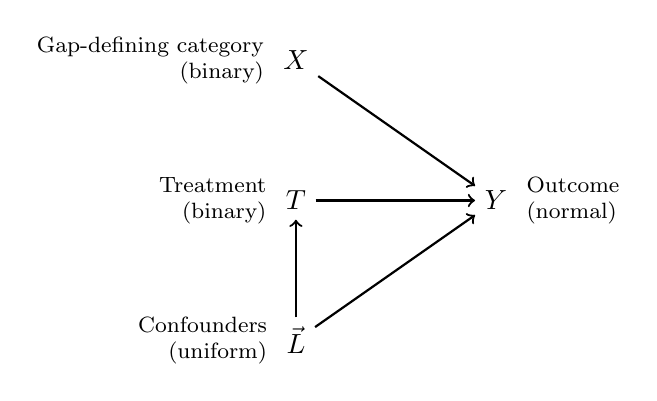
\begin{tikzpicture}[x = 1in, y = .7in]
\node (x) at (0,1) {$X$};
\node (t) at (0,0) {$T$};
\node (y) at (1,0) {$Y$};
\node (l) at (0,-1) {$\vec{L}$};
\draw[->, thick] (l) -- (y);
\draw[->, thick] (l) -- (t);
\draw[->, thick] (x) -- (y);
\draw[->, thick] (t) -- (y);
\node[font = \footnotesize, align = right, anchor = east] at (x.west) {Gap-defining category\\(binary)};
\node[font = \footnotesize, anchor = east, align = right, anchor = east] at (t.west) {Treatment\\(binary)};
\node[font = \footnotesize, anchor = east, align = right, anchor = east] at (l.west) {Confounders\\(uniform)};
\node[font = \footnotesize, anchor = west, align = left, anchor = west] at (y.east) {Outcome\\(normal)};
\end{tikzpicture}
\end{center}
\begin{itemize}
\item True outcome model is linear and additive
\item True treatment model is additive logistic regression
\end{itemize}
\end{frame}

\begin{frame}{Simulation details for cross-fitting}
\begin{align}
X&\sim \text{Bernoulli}(.5) \label{eq:sim2_eq1} \\
L_1,\dots,L_{10}&\sim \text{Uniform}(-1,1) \\
m(1,X,\vec{L}) &= \begin{cases}
        \text{logit}^{-1}\left(.1L_1 + \dots + .1L_{10}\right)
            &\text{ if }X = 1 \\
        \text{logit}^{-1}\left(.3L_1 + \dots + .3L_{10}\right)
            &\text{ if }X = 0 \\
    \end{cases} \\
T &\sim \text{Bernoulli}\left(m(1,X,\vec{L})\right) \\
g(T,X,\vec{L}) &= \begin{cases}
L_1 + \dots + L_{10} + T &\text{if }X = 1 \\
L_1 + \dots + L_{10} - T &\text{if }X = 0
\end{cases} \\
Y &\sim \text{Normal}\left(\text{Mean} = g(T,X,\vec{L}), \text{SD} = 10\right) \label{eq:sim2_eqN}
\end{align}
\end{frame}

\begin{frame}[t]
\label{description_misleading}
    \begin{tikzpicture}[x = \textwidth, y = .8\textheight]
    \node at (0,0) {};
    \node at (1,1) {};
    \node<1->[anchor = north east, draw = white, fill = gray, text = black, rounded corners, fill opacity = .2, text opacity = 1, align = left, font = \small] (quote) at (1,1) {It is the most surprising\\result of my career.\\};
    \node<1->[anchor = south east, font = \footnotesize] at (quote.south east) {--- Roland Fryer};
    \node<1->[anchor = north west] at (0,1) {\includegraphics[width = .5\textwidth, trim = {1in 6.5in 1in 1in}, clip]{figures/fryer_p1}};
    \node<2-7>[anchor = west, rotate = 6] at (0,.5) {\includegraphics[width = .5\textwidth]{figures/fryer_nytimes}};
    \node<3-7>[anchor = west, rotate = -8] at (0,.3) {\includegraphics[width = .5\textwidth]{figures/fryer_myth_wsj}};
    \node<4-7>[anchor = west, rotate = 3] at (0,.05) {\includegraphics[width = .5\textwidth]{figures/fryer_guardian}};
    % Perceived as black
    \node<5->[anchor = south, gray] at (.8,.7) {Perceived as \textbf{black}};
    \draw<5->[line width = 2pt, gray, line width = 2pt, rounded corners] (.65,.4) rectangle (.95,.7);
    \onslide<5>{
    \node[font = {\tiny\bf}, fill = red, rounded corners, line width = 1pt] at (.85,.65) {\textcolor{white}{Crime}};
    \node[font = {\tiny\bf}, fill = red, rounded corners, line width = 1pt] at (.85,.55) {\textcolor{white}{Crime}};
    \node[font = {\tiny\bf}, fill = gray, rounded corners, line width = 1pt] at (.75,.65) {\textcolor{white}{Safe}};
    \node[font = {\tiny\bf}, fill = gray, rounded corners, line width = 1pt] at (.75,.55) {\textcolor{white}{Safe}};
    \node[font = {\tiny\bf}, fill = gray, rounded corners, line width = 1pt] at (.85,.45) {\textcolor{white}{Safe}};
    \node[font = {\tiny\bf}, fill = gray, rounded corners, line width = 1pt] at (.75,.45) {\textcolor{white}{Safe}};
    }
    \onslide<6->{
    \node[draw = black, font = {\tiny\bf}, fill = red, rounded corners, line width = 1.5pt] at (.85,.65) {\textcolor{white}{Crime}};
    \node[draw = black, font = {\tiny\bf}, fill = red, rounded corners, line width = 1.5pt] at (.85,.55) {\textcolor{white}{Crime}};
    \node[draw = black, font = {\tiny\bf}, fill = gray, rounded corners, line width = 1.5pt] at (.75,.65) {\textcolor{white}{Safe}};
    \node[draw = black, font = {\tiny\bf}, fill = gray, rounded corners, line width = 1.5pt] at (.75,.55) {\textcolor{white}{Safe}};
    \node[opacity = .5, font = {\tiny\bf}, fill = gray, rounded corners, line width = 1.5pt] at (.85,.45) {\textcolor{white}{Safe}};
    \node[opacity = .5, font = {\tiny\bf}, fill = gray, rounded corners, line width = 1.5pt] at (.75,.45) {\textcolor{white}{Safe}};
    }
    % Perceived as white
    \node<5->[anchor = south, gray] at (.8,.3) {Perceived as \textbf{white}};
    \draw<5->[line width = 2pt, gray, line width = 2pt, rounded corners] (.65,0) rectangle (.95,.3);
    \onslide<5-6>{
    \node[font = {\tiny\bf}, fill = red, rounded corners, line width = 2pt] at (.85,.25) {\textcolor{white}{Crime}};
    \node[font = {\tiny\bf}, fill = red, rounded corners, line width = 1pt] at (.85,.15) {\textcolor{white}{Crime}};
    \node[font = {\tiny\bf}, fill = gray, rounded corners, line width = 1pt] at (.85,.05) {\textcolor{white}{Safe}};
    \node[font = {\tiny\bf}, fill = gray, rounded corners, line width = 1pt] at (.75,.25) {\textcolor{white}{Safe}};
    \node[font = {\tiny\bf}, fill = gray, rounded corners, line width = 1pt] at (.75,.15) {\textcolor{white}{Safe}};
    \node[font = {\tiny\bf}, fill = gray, rounded corners, line width = 1pt] at (.75,.05) {\textcolor{white}{Safe}};
    }
    \onslide<7->{
    \node[font = {\tiny\bf}, draw = black, fill = red, rounded corners, line width = 1.5pt] at (.85,.25) {\textcolor{white}{Crime}};
    \node[font = {\tiny\bf}, draw = black, fill = red, rounded corners, line width = 1.5pt] at (.85,.15) {\textcolor{white}{Crime}};
    \node[opacity = .5, font = {\tiny\bf}, fill = gray, rounded corners, line width = 1.5pt] at (.85,.05) {\textcolor{white}{Safe}};
    \node[opacity = .5, font = {\tiny\bf}, fill = gray, rounded corners, line width = 1.5pt] at (.75,.25) {\textcolor{white}{Safe}};
    \node[opacity = .5, font = {\tiny\bf}, fill = gray, rounded corners, line width = 1.5pt] at (.75,.15) {\textcolor{white}{Safe}};
    \node[opacity = .5, font = {\tiny\bf}, fill = gray, rounded corners, line width = 1.5pt] at (.75,.05) {\textcolor{white}{Safe}};
    }
    \node<8->[anchor = north west, align = left] at (.05,.5) {Equal use of force\\among those stopped\\is actually \bblue{consistent}\\with bias};
    \node<8->[anchor = south west, align = left, gray, font = \footnotesize] at (.05,0) {See Knox et al.~2020 for a fuller critique};
    \end{tikzpicture}
    \end{frame}

\begin{frame}
\includegraphics[width = \textwidth]{figures/sim_cross_fitting_convergence}
\end{frame}

\end{document}

% TAKEN FROM BEFORE DML SIM
\begin{frame}
\begin{tikzpicture}[x = \textwidth, y = .9\textheight]
\node at (0,0)  {};
\node at (1,1) {};
%\node[anchor = north west, font = \large] at (0,.95) {Estimation via outcome modeling};
% Factual science table is its own tikzppicture
\node[anchor = north west] (factual) at (0,.9) {
\scalebox{.5}{\begin{tikzpicture}[x = .8in, y = .3in, every node/.style={anchor = center}]
\node at (0,-4) {};
\node at (0,2) {};
\node at (0,-1) {Person 1};
\node at (0,-2) {Person 2};
\node at (0,-3) {Person 3};
\node at (0,-4.5) {Person 4};
\node at (0,-5.5) {Person 5};
\node at (0,-6.5) {Person 6};
\node[font = \bf, gray, align = center] at (-1.2,-2) {People in\\category 1};
\node[font = \bf, gray, align = center] at (-1.2,-5.5) {People in\\category 2};
\draw[line cap = round, gray, line width = 2pt] (-.5,-.6) -- (-.5,-3.4);
\draw[line cap = round, gray, line width = 2pt] (-.5,-4.1) -- (-.5,-6.9);
\node[anchor = south, align = center] at (1,0) {Outcome\\under\\treatment};
\node[anchor = south, align = center] at (2,0) {Outcome\\under\\control};
\node at (2,-1) {$Y_1$};
\node at (1,-2) {$Y_2$};
\node at (1,-3) {$Y_3$};
\node at (2,-4.5) {$Y_4$};
\node at (1,-5.5) {$Y_5$};
\node at (2,-6.5) {$Y_6$};
\node at (1,-1) {?};
\node at (2,-2) {?};
\node at (2,-3) {?};
\node at (1,-4.5) {?};
\node at (2,-5.5) {?};
\node at (1,-6.5) {?};
\only<2->{
\draw[color = white, fill = gray, opacity = .2, rounded corners] (.5,-3.5) rectangle (1.5,-.5);
\draw[color = white, fill = gray, opacity = .2, rounded corners] (.5,-7) rectangle (1.5,-4);
}
\end{tikzpicture}}
};
% End factual science table
\node<3->[anchor = south, font = \small] (factual_label) at (factual.north) {Learn a prediction function};
\draw<3->[gray, line width = 1.2pt, line cap = round] (factual_label.south west) -- (factual_label.south east);
% Predicted science table is its own tikzppicture
\node<4->[anchor = north west] (predicted) at (.5,.9) {
\scalebox{.5}{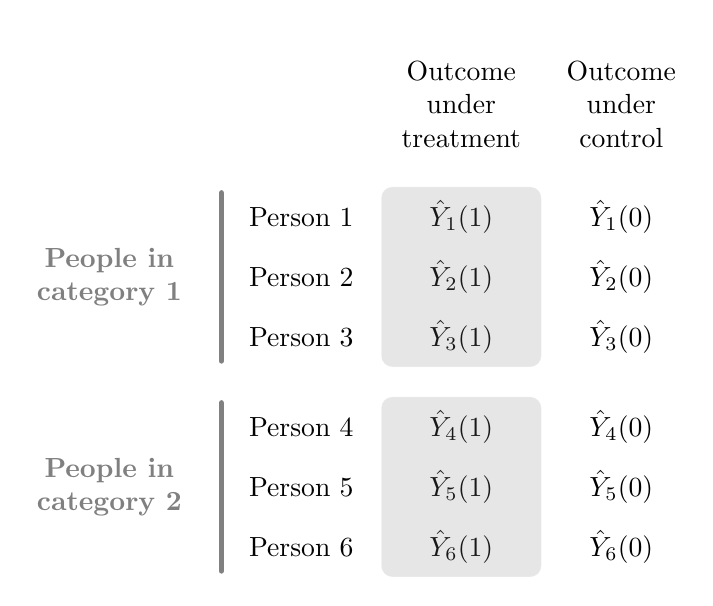
\begin{tikzpicture}[x = .8in, y = .3in, every node/.style={anchor = center}]
\node at (0,-4) {};
\node at (0,2) {};
\node at (0,-1) {Person 1};
\node at (0,-2) {Person 2};
\node at (0,-3) {Person 3};
\node at (0,-4.5) {Person 4};
\node at (0,-5.5) {Person 5};
\node at (0,-6.5) {Person 6};
\node[font = \bf, gray, align = center] at (-1.2,-2) {People in\\category 1};
\node[font = \bf, gray, align = center] at (-1.2,-5.5) {People in\\category 2};
\draw[line cap = round, gray, line width = 2pt] (-.5,-.6) -- (-.5,-3.4);
\draw[line cap = round, gray, line width = 2pt] (-.5,-4.1) -- (-.5,-6.9);
\node[anchor = south, align = center] at (1,0) {Outcome\\under\\treatment};
\node[anchor = south, align = center] at (2,0) {Outcome\\under\\control};
%%
\node at (2,-1) {$\hat{Y}_1(0)$};
\node at (1,-2) {$\hat{Y}_2(1)$};
\node at (1,-3) {$\hat{Y}_3(1)$};
\node at (2,-4.5) {$\hat{Y}_4(0)$};
\node at (1,-5.5) {$\hat{Y}_5(1)$};
\node at (2,-6.5) {$\hat{Y}_6(0)$};
%%
\node at (1,-1) {$\hat{Y}_1(1)$};
\node at (2,-2) {$\hat{Y}_2(0)$};
\node at (2,-3) {$\hat{Y}_3(0)$};
\node at (1,-4.5) {$\hat{Y}_4(1)$};
\node at (2,-5.5) {$\hat{Y}_5(0)$};
\node at (1,-6.5) {$\hat{Y}_6(1)$};
%%
\only<5->{
\draw[color = white, fill = gray, opacity = .2, rounded corners] (.5,-3.5) rectangle (1.5,-.5);
\draw[color = white, fill = gray, opacity = .2, rounded corners] (.5,-7) rectangle (1.5,-4);
}
\end{tikzpicture}}
};
% End predicted science table
\node<4->[anchor = south, font = \small] (predicted_label) at (predicted.north) {Predict the whole table};
\draw<4->[gray, line width = 1.2pt, line cap = round] (predicted_label.south west) -- (predicted_label.south east);
\node<4-5>[gray, font = \footnotesize, align  = right, anchor = south east] at (1,0) {Robins 1986\\Hahn 1998};
% Begin problem
\node<6->[anchor = south, font = \small] (problem) at (.5,.35) {Problem: Optimization for the wrong task};
\draw<6->[gray, line width = 1.2pt, line cap = round] (problem.south west) -- (problem.south east);
\node<7->[align = center, font = \footnotesize] at (.25,.25) {Prediction error over\\\bgray{observed}\\cases};
\node<8->[align = center, font = \footnotesize] at (.5,.25) {vs};
\node<8->[align = center, font = \footnotesize] at (.75,.25) {Prediction error over\\\bgray{all}\\cases};
\end{tikzpicture}
\end{frame}

\begin{frame}
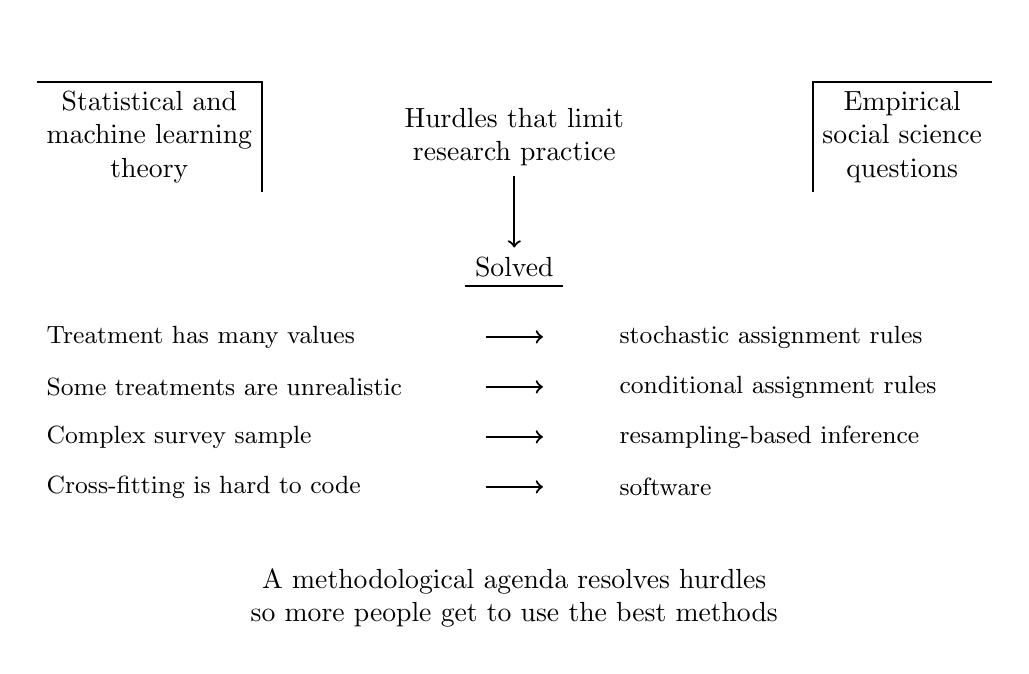
\begin{tikzpicture}[x = \textwidth, y = .5in]
\node at (0,-5) {};
\node at (1,1) {};
\node[align = center, anchor = west] (statistics) at (0,0) {Statistical and\\machine learning\\theory};
\node[align = center, anchor = east] (socialscience) at (1,0) {Empirical\\social science\\questions};
\draw[thick] (statistics.north west) -- (statistics.north east) -- (statistics.south east);
\draw[thick] (socialscience.north east) -- (socialscience.north west) -- (socialscience.south west);
\node<2->[align = center] (hurdles) at (.5,0) {Hurdles that limit\\research practice};
\node<3->[align = center] (solved) at (.5,-1.3) {Solved};
\draw<3->[->, thick]  (hurdles) -- (solved);
\draw<3->[thick] (solved.south west) -- (solved.south east);
%%%%
\node<4->[anchor = west, font = \small] at (0,-2) {Treatment has many values};
\draw<5->[->, thick] (.47,-2) -- (.53,-2);
\node<5->[anchor = west, font = \small] at (.6,-2) {stochastic assignment rules};
%%%%
\node<6->[anchor = west, font = \small] at (0,-2.5) {Some treatments are unrealistic};
\draw<7->[->, thick] (.47,-2.5) -- (.53,-2.5);
\node<7->[anchor = west, font = \small] at (.6,-2.5) {conditional assignment rules};
%%%%
\node<8->[anchor = west, font = \small] at (0,-3) {Complex survey sample};
\draw<9->[->, thick] (.47,-3) -- (.53,-3);
\node<9->[anchor = west, font = \small] at (.6,-3) {resampling-based inference};
%%%%
\node<10->[anchor = west, font = \small] at (0,-3.5) {Cross-fitting is hard to code};
\draw<11->[->, thick] (.47,-3.5) -- (.53,-3.5);
\node<11->[anchor = west, font = \small] at (.6,-3.5) {software};
\node<12->[align = center, anchor = south] at (.5,-5) {A methodological agenda resolves hurdles\\so more people get to use the best methods};
\end{tikzpicture}
\end{frame}

% HEALTH DISPARITIES VERSION IS BELOW

% Introduce gap-closing
\begin{frame}
\begin{tikzpicture}[x = \textwidth, y = \textheight]
\node at (0,0) {};
\node at (1,1) {};
%\node[align = right, anchor = east] at (1,.75) {Collections of units};
% Denote types of variables
%\node<1->[align = left, anchor = west, font = \small] at (0,.75) {Race\\Class Origin\\Gender};
% CATEGORIES
%\node[font = \footnotesize, align = center, anchor = south] (category1) at (.3,.85) {Gap-Defining\\Category\\$X = x$};
%\node[font = \footnotesize, align = center, anchor = south] (category2) at (.5,.85) {Gap-Defining\\Category\\$X = x'$};
%\draw[line width = 2pt, line cap = round, lightgray] (category1.south west) -- (category1.south east);
%\draw[line width = 2pt, line cap = round, lightgray] (category2.south west) -- (category2.south east);
\node[circle, fill = lightgray, draw = lightgray, font = \footnotesize, inner sep = 2pt] at (.42,.8) {\phantom{$t$}};
\node[circle, fill = lightgray, draw = lightgray, font = \footnotesize, inner sep = 2pt] at (.37,.75) {\phantom{$t$}};
\node[circle, fill = lightgray, draw = lightgray, font = \footnotesize, inner sep = 2pt] at (.42,.7) {\phantom{$t$}};
\node[diamond, fill = lightgray, draw = lightgray, font = \footnotesize, inner sep = 2pt] at (.58,.8) {\phantom{$t$}};
\node[diamond, fill = lightgray, draw = lightgray, font = \footnotesize, inner sep = 2pt] at (.63,.75) {\phantom{$t$}};
\node[diamond, fill = lightgray, draw = lightgray, font = \footnotesize, inner sep = 2pt] at (.58,.7) {\phantom{$t$}};
\only<2>{
\node[font = \bf, gray, align = center, anchor = north] (category1) at (.4,.95) {Working\\Class};
\node[font = \bf, gray, align = center, anchor = north] (category2) at (.6,.95) {Professional\\Class};
}
\only<3>{
\node[font = \bf, gray, align = center, anchor = south] (category1) at (.4,.85) {Men};
\node[font = \bf, gray, align = center, anchor = south] (category2) at (.6,.85) {Women};
}
\only<4->{
\node[font = \bf, gray, align = center, anchor = south] (category1) at (.4,.85) {Black};
\node[font = \bf, gray, align = center, anchor = south] (category2) at (.6,.85) {White};
}
%\node<5-6>[anchor = south east, align = right] (audit) at (.3,.5) {\bgray{Audit}\\\bgray{studies:}};
%\node<5-6>[anchor = north west, align = left] at (audit.north east) {What is the effect of \bblue{signaling}\\an identity as a circle versus a diamond?};
%\node<6>[anchor = north west, font = \small, gray, align = center] (audit_note) at (.25,.4) {Causal claims about\\one dimension of race};
%\draw<6>[->, thick, gray] (audit_note) to[bend left] (audit);
%\node<7-8>[anchor = south east, align = right] (descriptive) at (.3,.5) {\bgray{Descriptive}\\\bgray{studies:}};
%\node<7-8>[anchor = north west, align = left] at (descriptive.north east) {What is the disparity in outcomes\\between circles and diamonds};
%\node<8>[anchor = north west, font = \small, gray, align = center] (descriptive_note) at (.25,.4) {Non-causal claims\\about the whole of race};
%\draw<8>[->, thick, gray] (descriptive_note) to[bend left] (descriptive);
% TREATED
\only<5->{
\node[anchor = east, font = \small, gray, align = center] (treatment_note) at (.3,.6) {Give everyone\\a treatment $t$};
\draw[->, thick, gray] (treatment_note) to[bend right] (.33,.51);
\node[circle, fill = lightgray, draw = lightgray, font = \footnotesize, inner sep = 2pt] at (.42,.57) {$t$};
\node[circle, fill = lightgray, draw = lightgray, font = \footnotesize, inner sep = 2pt] at (.37,.52) {$t$};
\node[circle, fill = lightgray, draw = lightgray, font = \footnotesize, inner sep = 2pt] at (.42,.47) {$t$};
\node[diamond, fill = lightgray, draw = lightgray, font = \footnotesize, inner sep = 2pt] at (.58,.57) {$t$};
\node[diamond, fill = lightgray, draw = lightgray, font = \footnotesize, inner sep = 2pt] at (.63,.52) {$t$};
\node[diamond, fill = lightgray, draw = lightgray, font = \footnotesize, inner sep = 2pt] at (.58,.47) {$t$};
}
% Disparity
\only<6->{
\node[anchor = east, font = \small, gray, align = center] (disparity_note) at (.3,.31) {Is the disparity\\smaller?};
%\draw[->, thick, gray] (disparity_note) to[bend left] (.33,.29);
\node[circle, fill = lightgray, draw = lightgray, font = \footnotesize, inner sep = 2pt] at (.4,.31) {$\bar{y}(t)$};
\node[font = \footnotesize] at (.5,.31) {$-$};
\node[diamond, fill = lightgray, draw = lightgray, font = \footnotesize, inner sep = 2pt] at (.6,.31) {$\bar{y}(t)$};
}
\node[anchor = south east, font = \small, gray, align = right] at (1,.05) {\textbf{The Gap-Closing Estimand}\\A Causal Approach to Study Interventions\\That Close Disparities Across Social Categories};
%\node[anchor = south east, font = \small, gray, align = right] at (1,.05) {Lundberg, Ian\\Working paper\\On \bref{https://doi.org/10.31235/osf.io/gx4y3}{SocArxiv}};
\end{tikzpicture}
\end{frame}

% GAP-CLOSING PAST STUDIES
% Other examples
\begin{frame}
\begin{tikzpicture}[x = \textwidth, y = \textheight]
\node at (0,0) {};
\node at (1,1) {};
\node[font = \footnotesize] at (.15, .81) {\bgray{Categories}};
\node[font = \footnotesize] at (.45, .81) {\bgray{Treatment}};
\node[font = \footnotesize, align = center] at (.8, .81) {\bgray{Counterfactual Disparity}};
\node[circle, fill = lightgray, draw = lightgray, font = \footnotesize, inner sep = 2pt] at (.11,.95) {\phantom{$t$}};
\node[circle, fill = lightgray, draw = lightgray, font = \footnotesize, inner sep = 2pt] at (.11,.87) {\phantom{$t$}};
\node[diamond, fill = lightgray, draw = lightgray, font = \footnotesize, inner sep = 2pt] at (.19,.95) {\phantom{$t$}};
\node[diamond, fill = lightgray, draw = lightgray, font = \footnotesize, inner sep = 2pt] at (.19,.87) {\phantom{$t$}};
\node[circle, fill = lightgray, draw = lightgray, font = \footnotesize, inner sep = 2pt] at (.41,.95) {$t$};
\node[circle, fill = lightgray, draw = lightgray, font = \footnotesize, inner sep = 2pt] at (.41,.87) {$t$};
\node[diamond, fill = lightgray, draw = lightgray, font = \footnotesize, inner sep = 2pt] at (.49,.95) {$t$};
\node[diamond, fill = lightgray, draw = lightgray, font = \footnotesize, inner sep = 2pt] at (.49,.87) {$t$};
\node[circle, fill = lightgray, draw = lightgray, font = \footnotesize, inner sep = 2pt] at (.73,.91) {$\bar{y}(t)$};
\node[font = \footnotesize] at (.8,.91) {$-$};
\node[diamond, fill = lightgray, draw = lightgray, font = \footnotesize, inner sep = 2pt] at (.88,.91) {$\bar{y}(t)$};
%%%%%%%%%%%
% CHETTY  ET AL %
%%%%%%%%%%%
\node<8>[font = \footnotesize] at (.15, .77) {Parent Income};
\node<8>[font = \footnotesize] at (.45, .77) {Selective College};
\node<8>[font = \footnotesize] at (.8, .77) {Offspring Income};
\node<2-4> at (.5,.4) {\includegraphics[width = \textwidth]{figures/chetty_figure_1}};
\node<5> at (.5,.4) {\includegraphics[width = \textwidth]{figures/chetty_figure_2}};
\node<6-8> at (.5,.4) {\includegraphics[width = \textwidth]{figures/chetty_figure_3}};
\node<2-8>[anchor = south east, font = {\footnotesize\bf}, color = gray] at (1,.05) {Chetty et al. 2017};
\node<3-4>[anchor = north, font = \small] at (.5,.36) {The average child lands at the};
\node<3-4>[anchor = north west, align = left, font = \scriptsize] at (.1, .3) {\bblue{34th percentile} of income\\if their parents were at\\the \bblue{bottom} of the distribution};
\draw<3-4>[->, thick, blue] (.15,.3) to[bend left] (.15,.34);
\node<4>[anchor = north east, align = right, font = \scriptsize] at (.85, .3) {\bblue{65th percentile} of income\\if their parents were at\\the \bblue{top} of the distribution};
\draw<4>[->, thick, blue] (.83,.4) to[out = 90, in = 350] (.8,.5) to[out = 170, in = 0] (.77, .5);
\draw<7-8>[->, thick, seagreen4] (.173,.4) -- (.173, .51);
\draw<7-8>[->, thick, seagreen4] (.751,.52) -- (.751, .54);
%%%%%%%%
% WESTERN  %
%%%%%%%%
\node<10-13>[align = left, anchor = north west] (western1) at (.2, .6) {The difference in earnings};
\node<10-13>[align = left, anchor = north west] (western2) at (.2, .55) {between blacks and whites};
\node<11-13>[align = left, anchor = north west] (western3) at (.2, .5) {would be reduced only by about 3 percent};
\node<11-13>[align = left, anchor = north west] (western3) at (.2, .45) {if the incarceration rate were zero};
\node<10-13>[anchor = north west] at (.2,.37) {--- Western 2006:12};
\node<10-13>[font = \footnotesize] (race) at (.15, .77) {Race};
\draw<10>[->, line width = 1.2pt, gray] (.2,.53) to[bend left] (race);
\node<11-13>[font = \footnotesize] (earnings) at (.8, .77) {Earnings};
\draw<11>[->, line width = 1.2pt, gray] (.75,.5) to[bend right] (earnings);
\node<12-13>[font = \footnotesize] (incarceration) at (.45, .77) {Incarceration};
\draw<12>[->, line width = 1.2pt, gray] (.2,.43) to[out = 150, in = 200] (incarceration.south west);
%%%%%%%%%%%%%%%%%
% PETERSEN AND MORGAN  %
%%%%%%%%%%%%%%%%%
%\node<14-17>[align = left, anchor = north west] (western1) at (.15, .6) {Suppose sex segregation---by occupation,};
%\node<14-17>[align = left, anchor = north west] (western2) at (.15, .55) {establishment, or occupation-establishment};
%\node<14-17>[align = left, anchor = north west] (western3) at (.15, .5) {---were abolished; what then would the};
%\node<14-17>[align = left, anchor = north west] (western3) at (.15, .45) {remaining gender relative wages be?};
%\node<14-17>[anchor = north west] at (.15,.37) {--- Petersen and Morgan 1995:338};
%\node<15-17>[font = \footnotesize] (gender) at (.15, .77) {Gender};
%\node<16-17>[font = \footnotesize] (occupation) at (.45, .77) {Occupation-Establishment};
%\draw<16>[->, line width = 1.2pt, gray] (.45,.62) -- (occupation);
%\node<17>[font = \footnotesize] (wage) at (.8, .77) {Wage};
%\draw<17>[->, line width = 1.2pt, gray] (.73,.41) to[out = 10, in = 315] (wage);
%%%%%%%%%%%%%%
% We often want to know %
%%%%%%%%%%%%%%
\node<14->[align = left, anchor = west] at (.1,.5) {We often want to know\\if \bblue{intervening} on a treatment variable\\would close gaps};
\node<14>[anchor = south east, gray, align = center, font = \small] at (1,.05) {Jackson \& Vanderweele 2018};
\node<15->[align = left, anchor = west] at (.1,.3) {Would racial disparities narrow};
\node<15->[align = left, anchor = west] at (.1,.25) {if we eliminated occupational segregation?};
%\draw<20->[->, line width = 1.2pt, gray] (.6,.54) to[bend right] (.53,.74);
%\node<21->[align = left, anchor = north west, font = \small, gray] (causally) at (.6,.4) {Causally!};
%\draw<21->[->, thick, gray] (causally) -- (.5,.45);
\node<16->[font = \footnotesize] (gender) at (.15, .77) {Race};
\node<17->[font = \footnotesize] (wage) at (.8, .77) {Health};
\node<18->[font = \footnotesize] (occupation) at (.45, .77) {Occupation};
\end{tikzpicture}
\end{frame}

% MY HEALTH EXAMPLE
\begin{frame}
\label{descriptive_results}
\begin{tikzpicture}[x = \textwidth, y = \textheight]
\node at (0,0) {};
\node at (1,1) {};
\node<1->[anchor = north east, font = \footnotesize, align = right, gray] (note1) at (1,.65) {Current\\Population Survey\\Annual Social and\\Economic Supplement\\Ages 25--60\\2005--2020};
\node<2-17>[anchor = south west, align = left, text width = .87\textwidth, font = \footnotesize, fill = lightgray, fill opacity = .4, text opacity = 1, rounded corners] at (0,.8) {Do you have a health problem or disability which prevents you from working or which limits the kind or amount of work you can do?};
\node<3>[anchor = north west] at (0,.7) {\includegraphics[width = .68\textwidth]{figures/disability_by_race}};
% Timeline
\draw<4-6>[->, gray, line width = 2pt] (0,.5) -- (.65, .5);
\draw<4-6>[thick] (.15,.48) -- (.15, .52);
\draw<4-6>[thick] (.5,.48) -- (.5, .52);
\node<4-6>[anchor = south, font = \footnotesize] at (.15,.52) {Year $y$};
\node<4-6>[anchor = south, font = \footnotesize] at (.5,.52) {Year $y + 1$};
\node<5-6>[anchor = north, font = \footnotesize, align = center] at (.15,.48) {\bgray{Restriction}\\Employed with\\no work-limiting\\disability};
\node<6>[anchor = north, font = \footnotesize, align = center] at (.5,.48) {\bgray{Outcome}\\Onset of\\work-limiting\\disability};
% Onset results
\node<7>[anchor = north west] at (0,.7) {\includegraphics[width = .68\textwidth]{figures/onset_by_race}};
\node<7-18>[anchor = north east, font = \footnotesize, align = right, gray] at (note1.south east) {Employed last year\\No disability\\last year};
\node<7>[anchor = south west, align = left] at (.1,.7) {\textbf{Onset of Work-Limiting Disability}};
\node<8>[anchor = north west] at (0,.7) {\includegraphics[width = .68\textwidth]{figures/scatter_factual_outcome_re_NonHispanicBlack_slide1}};
\node<9>[anchor = north west] at (0,.7) {\includegraphics[width = .68\textwidth]{figures/scatter_factual_outcome_re_NonHispanicBlack_slide2}};
\node<10>[anchor = north west] at (0,.7) {\includegraphics[width = .68\textwidth]{figures/scatter_factual_outcome_re_NonHispanicBlack_slide3}};
\node<11>[anchor = north west] at (0,.7) {\includegraphics[width = .68\textwidth]{figures/scatter_factual_outcome_re_NonHispanicBlack_slide4}};
\node<12>[anchor = north west] at (0,.7) {\includegraphics[width = .68\textwidth]{figures/scatter_factual_outcome_re_NonHispanicBlack_slide5}};
\node<13>[anchor = north west] at (0,.7) {\includegraphics[width = .68\textwidth]{figures/scatter_factual_outcome_re_NonHispanicBlack_slide6}};
\node<14->[anchor = north west] at (0,.7) {\includegraphics[width = .3\textwidth]{figures/scatter_factual_outcome_re_NonHispanicBlack_annotated}};
\node<15->[anchor = north west] at (0,.4) {\includegraphics[width = .3\textwidth]{figures/scatter_factual_outcome_re_Hispanic_annotated}};
\node<16->[anchor = north west] at (.35,.7) {\includegraphics[width = .3\textwidth]{figures/scatter_factual_outcome_re_NonHispanicWhite_annotated}};
\node<17->[anchor = north west] at (.35,.4) {\includegraphics[width = .3\textwidth]{figures/scatter_factual_outcome_re_Other_annotated}};
\node<18>[anchor = south west, align = left] at (0,.8) {To what degree does \bblue{occupational segregation}\\contribute to \bblue{racial health disparities}?};
\end{tikzpicture}
\end{frame}

% Structure of the talk
\begin{frame}
\begin{tikzpicture}[x = \textwidth, y = \textheight]
\node at (0,0) {};
\node at (1,1) {};
\node[anchor = west, align = left] (gce) at (0.2, .9) {The \bblue{gap-closing estimand}:};
\node[anchor = west, align = left] (categories) at (0.2,.85) {The disparity across \bgreen{social categories}};
\node[anchor = west, align = left] (treatment) at (0.2,.8) {that would persist if we \bgreen{equalized a treatment}};
\node[anchor = east, align = right] at (.15, .88) {\bgray{General}};
\node[anchor = east, align = right] at (.15, .83) {\bgray{method}};
\draw[line width = 2pt, gray, line cap = round] (.175,.78) -- (.175,.93);
\node[anchor = west, align = left] (gce) at (.2, .7) {Occupational segregation contributes};
\node[anchor = west, align = left] (categories) at (.2,.65) {to racial disparities in health};
\node[anchor = east, align = right] at (.15, .7) {\bgray{Specific}};
\node[anchor = east, align = right] at (.15, .65) {\bgray{example}};
\draw[line width = 2pt, gray, line cap = round] (.175,.73) -- (.175,.63);
\node (plan) at (.5,.53) {\bgray{Structure of the talk}};
\draw[line width = 2pt, gray, line cap = round] (plan.south west) -- (plan.south east);
\node[anchor = west] at (.04,.44) {\bgray{Introduction}};
\node[anchor = west] at (.04,.38) {\bgray{Data}};
\node[anchor = west] at (.04,.32) {\bgray{Causal Question}};
\node[anchor = west] at (.04,.26) {\bgray{Estimation}};
\node[anchor = west] at (.04,.2) {\bgray{Results}};
\node[anchor = west] at (.04,.14) {\bgray{Research Agenda}};
\node[anchor = west] at (.35,.44) {Disparities call for explanations};
\node[anchor = west] at (.35,.38) {Current Population Survey};
\node[anchor = west] at (.35,.32) {How an intervention would close a gap};%change a disparity};
\node[anchor = west] at (.35,.26) {Causal assumptions and predictive tools};
\node[anchor = west] at (.35,.2) {Partially closing a gap in health};
\node[anchor = west] at (.35,.14) {Developing methods for new questions};
\draw[->, line width = 2pt, gray] (0,.38) -- (.04, .38);
\end{tikzpicture}
\end{frame}

\section{Causal Question}

% FROM AMONG TO WOULD
\begin{frame}
\begin{tikzpicture}[x = \textwidth, y = .8\textheight]
\node at (.05,-.1) {};
\node at (1,1) {};
\node<1->[anchor = north west] at (.05,1.1) {\phantom{From \bgray{among} statements to \bgray{would} statements}};
%\node<25-31>[anchor = north west] at (.05,1.1) {From \bgray{among} statements to \bgray{would} statements};
% Set up the table
\only<1->{
\node[anchor = east, font = \footnotesize] at (.2, .8) {Person 1};
\node[anchor = east, font = \footnotesize] at (.2, .7) {Person 2};
\node[anchor = east, font = \footnotesize] at (.2, .6) {Person 3};
\node[anchor = east, font = \footnotesize] at (.2, .5) {Person 4};
\node[anchor = east, font = \footnotesize] at (.2, .4) {Person 5};
\node[anchor = east, font = \footnotesize] at (.2, .3) {Person 6};
\node[anchor = east, font = \footnotesize] at (.2, .2) {Person 7};
\node[anchor = east, font = \footnotesize] at (.2, .1) {Person 8};
}
\only<1->{
\node[anchor = south, font = \footnotesize, align = center] at (.3, .85) {Administrative\\Assistant};
\node[anchor = south, font = \footnotesize, align = center] at (.5, .85) {Home Health\\Aid};
\node[anchor = south, font = \footnotesize, align = center] at (.7, .85) {Sales\\Supervisor};
}
% Place the factual occupations first
\node<1->[draw, line width = 1pt, circle, fill = lightgray, fill opacity = 1, inner sep = 4pt] (1a) at (.3, .8) {};
\node<1->[draw, line width = 1pt, circle, fill = lightgray, fill opacity = 1, inner sep = 4pt] (2a) at (.3, .7) {};
\node<1->[draw, line width = 1pt, circle, fill = lightgray, fill opacity = 1, inner sep = 4pt] (3b) at (.5, .6) {};
\node<1->[draw, line width = 1pt, circle, fill = lightgray, fill opacity = 1, inner sep = 4pt] (4c) at (.7, .5) {};
\draw<1->[thick, dashed] (.05,.45) -- (.75,.45);
\node<1->[draw, line width = 1pt, diamond, fill = lightgray, fill opacity = 1, inner sep = 4pt] (5b) at (.5, .4) {};
\node<1->[draw, line width = 1pt, diamond, fill = lightgray, fill opacity = 1, inner sep = 4pt] (6c) at (.7, .3) {};
\node<1->[draw, line width = 1pt, diamond, fill = lightgray, fill opacity = 1, inner sep = 4pt] (7b) at (.5, .2) {};
\node<1->[draw, line width = 1pt, diamond, fill = lightgray, fill opacity = 1, inner sep = 4pt] (8a) at (.3, .1) {};
% Create the legend for sick and healthy
\only<2-9>{
\node[anchor = west, font = \bf] at (.9,.5) {Legend};
\draw[thick] (.8,.05) -- (.8,.55) -- (1.1,.55);
\node[anchor = east] at (.9,.4) {\textcolor{seagreen4}{$\checkmark$}};
\node[anchor = east] at (.9,.3) {\includegraphics[width = 10pt]{figures/injury}};
\node[anchor = west] at (.9,.4) {Healthy};
\node[anchor = west] at (.9,.3) {Sick};
}
% Place the health conditions on those
\node<2->[seagreen4] at (1a) {$\checkmark$};
\node<2->[seagreen4] at (2a) {$\checkmark$};
\node<2-> at (3b) {\includegraphics[width = 10pt]{figures/injury}};
\only<2->{
\node[seagreen4] at (4c) {$\checkmark$};
\node at (5b) {\includegraphics[width = 10pt]{figures/injury}};
\node[seagreen4] at (6c) {$\checkmark$};
\node at (7b) {\includegraphics[width = 10pt]{figures/injury}};
\node at (8a) {\includegraphics[width = 10pt]{figures/injury}};
}
% Do the total disparity
\node<3-4>[red, font = \bf, draw, line width = 2pt, rounded corners] at (.6,.75) {1 / 4 sick};
\node<4>[red, font = \bf, draw, line width = 2pt, rounded corners] at (.6, .1) {3 / 4 sick};
% Do the conditional disparity
\draw<5>[fill = lightgray, fill opacity = .2] (.4,.05) rectangle (.6,.98);
\node<5>[anchor = north, align = center, font = \footnotesize] at (.5,.05) {No disparity \bgray{among}\\home health aids};
% Begin causal with row 1
\node<6->[circle, fill = lightgray, fill opacity = 1, inner sep = 4pt] (1b) at (.5, .8) {};
\node<7-> at (1b) {\includegraphics[width = 10pt]{figures/injury}};
% Create the legend for observed and unobserved
\only<8-9>{
\node[anchor = east, draw, line width = 1pt, diamond, fill = lightgray, fill opacity = 1, inner sep = 4pt] (obsDiamond) at (.9,.2) {};
\node[anchor = east, draw, line width = 1pt, circle, fill = lightgray, fill opacity = 1, inner sep = 4pt] (obsCircle) at (obsDiamond.west) {};
\node[anchor = west] at (.9,.2) {Observed};
\node[anchor = east, diamond, fill = lightgray, fill opacity = 1, inner sep = 4pt] (unobsDiamond) at (.9,.1) {};
\node[anchor = east, circle, fill = lightgray, fill opacity = 1, inner sep = 4pt] (unobsCircle) at (unobsDiamond.west) {};
\node[anchor = west] at (.9,.1) {Unobserved};
\node[anchor = south east, gray] at (1.1,-.07) {Imbens and Rubin 2015};
}
\only<8->{
\node<8->[circle, fill = lightgray, fill opacity = 1, inner sep = 4pt] (1c) at (.7, .8) {};
\node<8->[seagreen4] at (1c) {$\checkmark$};
% Add person 2 counterfactuals
\node[circle, fill = lightgray, fill opacity = 1, inner sep = 4pt] (2b) at (.5, .7) {};
\node[circle, fill = lightgray, fill opacity = 1, inner sep = 4pt] (2c) at (.7, .7) {};
\node[seagreen4] at (2b) {$\checkmark$};
\node[seagreen4] at (2c) {$\checkmark$};
% Add all others' counterfactuals
\node[circle, fill = lightgray, fill opacity = 1, inner sep = 4pt] (3a) at (.3, .6) {};
\node[circle, fill = lightgray, fill opacity = 1, inner sep = 4pt] (3c) at (.7, .6) {};
\node at (3a) {\includegraphics[width = 10pt]{figures/injury}};
\node[seagreen4] at (3c) {$\checkmark$};
\node[circle, fill = lightgray, fill opacity = 1, inner sep = 4pt] (4a) at (.3, .5) {};
\node[circle, fill = lightgray, fill opacity = 1, inner sep = 4pt] (4b) at (.5, .5) {};
\node[seagreen4] at (4a) {$\checkmark$};
\node[seagreen4] at (4b) {$\checkmark$};
\node[diamond, fill = lightgray, fill opacity = 1, inner sep = 4pt] (5a) at (.3, .4) {};
\node[diamond, fill = lightgray, fill opacity = 1, inner sep = 4pt] (5c) at (.7, .4) {};
\node[seagreen4] at (5a) {$\checkmark$};
\node[seagreen4] at (5c) {$\checkmark$};
\node[diamond, fill = lightgray, fill opacity = 1, inner sep = 4pt] (6a) at (.3, .3) {};
\node[diamond, fill = lightgray, fill opacity = 1, inner sep = 4pt] (6b) at (.5, .3) {};
\node[seagreen4] at (6a) {$\checkmark$};
\node at (6b) {\includegraphics[width = 10pt]{figures/injury}};
\node[diamond, fill = lightgray, fill opacity = 1, inner sep = 4pt] (7a) at (.3, .2) {};
\node[diamond, fill = lightgray, fill opacity = 1, inner sep = 4pt] (7c) at (.7, .2) {};
\node at (7a) {\includegraphics[width = 10pt]{figures/injury}};
\node[seagreen4] at (7c) {$\checkmark$};
\node[diamond, fill = lightgray, fill opacity = 1, inner sep = 4pt] (8b) at (.5, .1) {};
\node at (8b) {\includegraphics[width = 10pt]{figures/injury}};
\node[diamond, fill = lightgray, fill opacity = 1, inner sep = 4pt] (8c) at (.7, .1) {};
\node[seagreen4] at (8c) {$\checkmark$};
}
% AFTER 31, LEGEND IS GONE
% STOCHASTIC TREATMENT BEGINS
\node<9->[anchor = north west] at (.05,1.1) {What if occupations were \bgray{assigned at random}?};
% Average for each circle
\node<10->[font = {\footnotesize\bf}, anchor = south, align = center] at (.87,.85) {Probability\\of Sickness};
\node<10-> at (.87,.8) {1 / 3};
\node<10-> at (.87,.7) {0 / 3};
\node<10-> at (.87,.6) {2 / 3};
\node<10-> at (.87,.5) {0 / 3};
% Average for each diamond
\node<10-> at (.87,.4) {1 / 3};
\node<10-> at (.87,.3) {1 / 3};
\node<10-> at (.87,.2) {2 / 3};
\node<10-> at (.87,.1) {2 / 3};
% Average for all circles
\node<11->[draw, circle] at (1,.65) {$\frac{3}{12}$};
% Average for all diamonds
\node<11->[draw, diamond, inner sep = 2pt] at (1,.25) {$\frac{6}{12}$};
% Difference
\node<12->[anchor = east, font = {\footnotesize\bf}, gray] at (.6, .02) {Counterfactual Disparity:};
\only<12->{
\node[draw, diamond, inner sep = 0pt, font = \footnotesize] at (.65,.02) {$\frac{6}{12}$};
\node[font = \footnotesize] at (.725,.02) {$-$};
\node[draw, circle, inner sep = 0pt, font = \footnotesize] at (.8,.02) {$\frac{3}{12}$};
\node[anchor = west, font = \footnotesize] at (.85,.02) {$=\frac{3}{12}$};
\node[anchor = west, font = \footnotesize] at (.95,.02) {$=25\%$};
}
\node<13->[anchor = east, font = {\footnotesize\bf}, gray] at (.6, -.07) {Factual Disparity:};
\only<13-15>{
\node[draw, diamond, inner sep = 0pt, font = \footnotesize] at (.65,-.07) {$\frac{3}{4}$};
\node[font = \footnotesize] at (.725,-.07) {$-$};
\node[draw, circle, inner sep = 0pt, font = \footnotesize] at (.8,-.07) {$\frac{1}{4}$};
\node[anchor = west, font = \footnotesize] at (.85,-.07) {$=\frac{1}{2}$};
\node[anchor = west, font = \footnotesize] at (.95,-.07) {$=50\%$};
}
\only<14>{
	\node[circle, fill = white, draw = white, inner sep = 4pt] at (1b) {};
	\node[circle, fill = white, draw = white, inner sep = 4pt] at (1c) {};
	\node[circle, fill = white, draw = white, inner sep = 4pt] at (2b) {};
	\node[circle, fill = white, draw = white, inner sep = 4pt] at (2c) {};
	\node[circle, fill = white, draw = white, inner sep = 4pt] at (3a) {};
	\node[circle, fill = white, draw = white, inner sep = 4pt] at (3c) {};
	\node[circle, fill = white, draw = white, inner sep = 4pt] at (4a) {};
	\node[circle, fill = white, draw = white, inner sep = 4pt] at (4b) {};
	\node[diamond, fill = white, draw = white, inner sep = 4pt] at (5a) {};
	\node[diamond, fill = white, draw = white, inner sep = 4pt] at (5c) {};
	\node[diamond, fill = white, draw = white, inner sep = 4pt] at (6a) {};
	\node[diamond, fill = white, draw = white, inner sep = 4pt] at (6b) {};
	\node[diamond, fill = white, draw = white, inner sep = 4pt] at (7a) {};
	\node[diamond, fill = white, draw = white, inner sep = 4pt] at (7c) {};
	\node[diamond, fill = white, draw = white, inner sep = 4pt] at (8b) {};
	\node[diamond, fill = white, draw = white, inner sep = 4pt] at (8c) {};
}
\end{tikzpicture}
\end{frame}

\begin{frame}
\bgray{Key problem:} Predicting where we don't have data.
\begin{itemize}
\item Need assumptions for causal identification
\item Need to update machine learning to the correct loss function
\end{itemize}
\end{frame}

\begin{frame}
\label{dag}
\begin{tikzpicture}[x = \textwidth, y = \textheight]
\node at (0,0) {};
\node at (1,1) {};
\node[anchor = north west, align = left] at (0,.95) {\bblue{Identification:}};
%\node[anchor = north west, align = left] at (.25,.95) {We have to impute the outcome each person $i$\\would realize in each occupation $t$};
\node<1>[anchor = east, align = left, font = \small, gray] at (1,.1) {Pearl 2009, Morgan \& Winship 2015, Hern\'an \& Robins 2020};
\node<1,3-> (l) at (.3,.5) {$\vec{L}$};
\node<2>[draw, rounded corners] (l) at (.3,.5) {$\vec{L}$};
\node<1,3-> (x) at (.3,.7) {Race};
\node<2>[draw, rounded corners] (x) at (.3,.7) {Race};
\node<1-> (t) at (.5,.6) {Occupation};
\node<1-> (y) at (.75,.6) {Health};
\node<1->[anchor = north, font = \footnotesize, align = center] (predictors) at (l.south west) {Predictors};
\draw<1->[->, thick] (l) -- (t);
\draw<1->[->, thick] (l) to[bend right = 15] (y);
\draw<1->[->, line width = 2pt, blue] (t) -- (y);
\draw<1-6,8->[->, thick] (x) -- (t);
\draw<1-6,8->[->, thick] (x) -- (l);
\draw<1-6,8->[->, thick] (x) to[bend left = 40] (y);
% Confounding of T is bad
\node<3,10>[red] (u) at (.5,.4) {$U$};
\draw<3,10>[->, red, line width = 2pt] (u) -- (t);
\draw<3,10>[->, red, line width = 2pt] (u) to[bend right = 20] (y); 
% Confounding of X is ok
\node<4>[seagreen4] (v) at (.15,.4) {$V$};
\draw<4>[->, seagreen4, line width = 2pt] (v) to[bend left = 20] (x);
\draw<4>[->, seagreen4, line width = 2pt] (v) to[out = 0, in = 240] (y); 
% Agnostic about causal effect of X
\node<5-8>[anchor = west, align = left] at (0,.35) {A gap-closing estimand is \bblue{agnostic} about the causal effect of race};
\node<6-8>[anchor = west, align = left, font = \small] at (0,.28) {--- Race can affect everything};
\node<7-8>[anchor = west, align = left, font = \small] at (0,.22) {--- Race can have no causal effects};
\node<8>[anchor = west, align = left, font = \small] at (0,.16) {--- The effect of race can be philosophically complex};
\node<6>[anchor = east, align = left, font = \small, gray] at (1,.1) {Williams et al. 2019};
\node<7>[anchor = east, align = left, font = \small, gray] at (1,.1) {Greiner \& Rubin 2011};
\node<8>[anchor = east, align = left, font = \small, gray] at (1,.1) {Sen \& Wasow 2016, Kohler-Hausmann 2018};
\node<9-10>[anchor = north west, align = left, font = \footnotesize] at (predictors.south west) {Race\\Sex\\Education\\Foreign born\\Never left a job for health reasons\\Lagged outcome};
\draw<9-10>[thick] (predictors.south west) -- (predictors.south east);
\end{tikzpicture}
\end{frame}

% HOW TO ESTIMATE
\begin{frame}
\begin{tikzpicture}[x = \textwidth, y = \textheight]
\node at (0,0) {};
\node at (1,1) {};
\node[anchor = north] (how) at (.5, .95) {How to estimate a gap-closing estimand};
\draw[line width = 2pt, gray, line cap = round] (how.south west) -- (how.south east);
% Some shading boxes that appear later
% but are coded here so that text appears on top of them
\draw<18-20>[fill = lightgray, fill opacity = .5, rounded corners, draw = lightgray] (0,.425) rectangle (1,.475);
\draw<21>[fill = lightgray, fill opacity = .5, rounded corners, draw = lightgray] (0,.375) rectangle (1,.425);
\draw<22>[fill = lightgray, fill opacity = .5, rounded corners, draw = lightgray] (0,.325) rectangle (1,.375);
\draw<23>[fill = lightgray, fill opacity = .5, rounded corners, draw = lightgray] (0,.275) rectangle (1,.325);
\draw<24>[fill = lightgray, fill opacity = .5, rounded corners, draw = lightgray] (0,.225) rectangle (1,.275);
\draw<25>[fill = lightgray, fill opacity = .5, rounded corners, draw = lightgray] (0,.175) rectangle (1,.225);
\draw<26>[fill = lightgray, fill opacity = .5, rounded corners, draw = lightgray] (0,.125) rectangle (1,.175);
\draw<27>[fill = lightgray, fill opacity = .5, rounded corners, draw = lightgray] (0,.075) rectangle (1,.125);
\draw<29>[fill = lightgray, fill opacity = .5, rounded corners, draw = lightgray] (.85,.275) rectangle (.95,.475);
\draw<31>[fill = lightgray, fill opacity = .5, rounded corners, draw = lightgray] (.85,.075) rectangle (.95,.275);
\only<2->{
% Begin science table
\node[anchor = east, font = \footnotesize] at (.2, .45) {Person 1};
\node[anchor = east, font = \footnotesize] at (.2, .4) {Person 2};
\node[anchor = east, font = \footnotesize] at (.2, .35) {Person 3};
\node[anchor = east, font = \footnotesize] at (.2, .3) {Person 4};
\node[anchor = east, font = \footnotesize] at (.2, .25) {Person 5};
\node[anchor = east, font = \footnotesize] at (.2, .2) {Person 6};
\node[anchor = east, font = \footnotesize] at (.2, .15) {Person 7};
\node[anchor = east, font = \footnotesize] at (.2, .1) {Person 8};
\node[anchor = south, font = \footnotesize, align = center] at (.3, .5) {Administrative\\Assistant};
\node[anchor = south, font = \footnotesize, align = center] at (.5, .5) {Home Health\\Aid};
\node[anchor = south, font = \footnotesize, align = center] at (.7, .5) {Sales\\Supervisor};
% Factual occupations first
\node[draw, line width = 1pt, circle, fill = lightgray, fill opacity = 1, inner sep = 3pt] (1a) at (.3, .45) {};
\node[draw, line width = 1pt, circle, fill = lightgray, fill opacity = 1, inner sep = 3pt] (2a) at (.3, .4) {};
\node[draw, line width = 1pt, circle, fill = lightgray, fill opacity = 1, inner sep = 3pt] (3b) at (.5, .35) {};
\node[draw, line width = 1pt, circle, fill = lightgray, fill opacity = 1, inner sep = 3pt] (4c) at (.7, .3) {};
\draw[thick, dashed] (.05,.275) -- (.75,.275);
\node[draw, line width = 1pt, diamond, fill = lightgray, fill opacity = 1, inner sep = 3pt] (5b) at (.5, .25) {};
\node[draw, line width = 1pt, diamond, fill = lightgray, fill opacity = 1, inner sep = 3pt] (6c) at (.7, .2) {};
\node[draw, line width = 1pt, diamond, fill = lightgray, fill opacity = 1, inner sep = 3pt] (7b) at (.5, .15) {};
\node[draw, line width = 1pt, diamond, fill = lightgray, fill opacity = 1, inner sep = 3pt] (8a) at (.3, .1) {};
}
% Counterfactual occupations
\only<2,9->{
\node[circle, fill = lightgray, fill opacity = 1, inner sep = 3pt] (3a) at (.3, .35) {};
\node[circle, fill = lightgray, fill opacity = 1, inner sep = 3pt] (4a) at (.3, .3) {};
\node[diamond, fill = lightgray, fill opacity = 1, inner sep = 3pt] (5a) at (.3, .25) {};
\node[diamond, fill = lightgray, fill opacity = 1, inner sep = 3pt] (6a) at (.3, .2) {};
\node[diamond, fill = lightgray, fill opacity = 1, inner sep = 3pt] (7a) at (.3, .15) {};
}
\only<2,12->{
\node[circle, fill = lightgray, fill opacity = 1, inner sep = 3pt] (1b) at (.5, .45) {};
\node[circle, fill = lightgray, fill opacity = 1, inner sep = 3pt] (2b) at (.5, .4) {};
\node[circle, fill = lightgray, fill opacity = 1, inner sep = 3pt] (4b) at (.5, .3) {};
\node[diamond, fill = lightgray, fill opacity = 1, inner sep = 3pt] (6b) at (.5, .2) {};
\node[diamond, fill = lightgray, fill opacity = 1, inner sep = 3pt] (8b) at (.5, .1) {};
}
\only<2,15->{
\node[circle, fill = lightgray, fill opacity = 1, inner sep = 3pt] (1c) at (.7, .45) {};
\node[circle, fill = lightgray, fill opacity = 1, inner sep = 3pt] (2c) at (.7, .4) {};
\node[circle, fill = lightgray, fill opacity = 1, inner sep = 3pt] (3c) at (.7, .35) {};
\node[diamond, fill = lightgray, fill opacity = 1, inner sep = 3pt] (5c) at (.7, .25) {};
\node[diamond, fill = lightgray, fill opacity = 1, inner sep = 3pt] (7c) at (.7, .15) {};
\node[diamond, fill = lightgray, fill opacity = 1, inner sep = 3pt] (8c) at (.7, .1) {};
}
% Counterfactual question marks
\only<2>{
\node[font = \tiny] at (1b) {?};
\node[font = \tiny] at (1c) {?};
\node[font = \tiny] at (2b) {?};
\node[font = \tiny] at (2c) {?};
\node[font = \tiny] at (3a) {?};
\node[font = \tiny] at (3c) {?};
\node[font = \tiny] at (4a) {?};
\node[font = \tiny] at (4b) {?};
\node[font = \tiny] at (5a) {?};
\node[font = \tiny] at (5c) {?};
\node[font = \tiny] at (6a) {?};
\node[font = \tiny] at (6b) {?};
\node[font = \tiny] at (7a) {?};
\node[font = \tiny] at (7c) {?};
\node[font = \tiny] at (8b) {?};
\node[font = \tiny] at (8c) {?};
}
% Begin prediction function
\node<4-16>[draw = gray, line width = 1.2pt, rounded corners, align = center] at (.5,.73) {Prediction\\Function};
\node<5-16>[anchor = south] (input) at (.2,.78) {Input};
\draw<5-16>[thick] (input.south west) -- (input.south east);
\node<5-6,16>[font = \footnotesize, align = center, anchor = north] at (.2,.78) {$\text{Covariates}_i$\\$\text{Occupation}_i$};
\draw<5-16>[->, thick] (.3,.73) -- (.37,.73);
\node<6-16>[anchor = south] (output) at (.8,.78) {Output};
\draw<6-16>[thick] (output.south west) -- (output.south east);
\node<6-16>[font = \footnotesize, align = center, anchor = north] (predicted) at (.8,.78) {Predicted\\$\text{Health}_i$};
\draw<6-16>[->, thick] (.63,.73) -- (.7,.73);
% Make the input administrative assistant
\node<7-9>[font = \footnotesize, align = center, anchor = north] at (.2,.78) {$\text{Covariates}_i$\\$\substack{\texttt{Administrative}\\\texttt{Assistant}}$};
\node<8-9>[font = \footnotesize, align = center, anchor = west] at (predicted.east) {$\left(\substack{\text{as an}\\\texttt{Administrative}\\\texttt{Assistant}}\right)$};
\only<9->{
\node[font = \tiny] at (1a) {$\hat{y}$};
\node[font = \tiny] at (2a) {$\hat{y}$};
\node[font = \tiny] at (3a) {$\hat{y}$};
\node[font = \tiny] at (4a) {$\hat{y}$};
\node[font = \tiny] at (5a) {$\hat{y}$};
\node[font = \tiny] at (6a) {$\hat{y}$};
\node[font = \tiny] at (7a) {$\hat{y}$};
\node[font = \tiny] at (8a) {$\hat{y}$};
}
% Make the input home health aid
\node<10-12>[font = \footnotesize, align = center, anchor = north] at (.2,.78) {$\text{Covariates}_i$\\$\substack{\texttt{Home Health}\\\texttt{Aid}}$};
\node<11-12>[font = \footnotesize, align = center, anchor = west] at (predicted.east) {$\left(\substack{\text{as a}\\\texttt{Home Health}\\\texttt{Aid}}\right)$};
\only<12->{
\node[font = \tiny] at (1b) {$\hat{y}$};
\node[font = \tiny] at (2b) {$\hat{y}$};
\node[font = \tiny] at (3b) {$\hat{y}$};
\node[font = \tiny] at (4b) {$\hat{y}$};
\node[font = \tiny] at (5b) {$\hat{y}$};
\node[font = \tiny] at (6b) {$\hat{y}$};
\node[font = \tiny] at (7b) {$\hat{y}$};
\node[font = \tiny] at (8b) {$\hat{y}$};
}
% Make the input sales supervisor
\node<13-15>[font = \footnotesize, align = center, anchor = north] at (.2,.78) {$\text{Covariates}_i$\\$\substack{\texttt{Sales}\\\texttt{Supervisor}}$};
\node<14-15>[font = \footnotesize, align = center, anchor = west] at (predicted.east) {$\left(\substack{\text{as a}\\\texttt{Sales}\\\texttt{Supervisor}}\right)$};
\only<15->{
\node[font = \tiny] at (1c) {$\hat{y}$};
\node[font = \tiny] at (2c) {$\hat{y}$};
\node[font = \tiny] at (3c) {$\hat{y}$};
\node[font = \tiny] at (4c) {$\hat{y}$};
\node[font = \tiny] at (5c) {$\hat{y}$};
\node[font = \tiny] at (6c) {$\hat{y}$};
\node[font = \tiny] at (7c) {$\hat{y}$};
\node[font = \tiny] at (8c) {$\hat{y}$};
}
\node<16>[font = \small, anchor = south east, gray, align = right] at (1,.1) {Robins 1986\\Hahn 1998};
\node<19->[anchor = south, font = \footnotesize, align = center] at (.9,.5) {Probability\\of Disability\\in an Equitable\\Occupation Lottery};
\node<20-29> at (.9,.45) {0.02};
\node<21-29> at (.9,.4) {0.01};
\node<22-29> at (.9,.35) {0.02};
\node<23-29> at (.9,.3) {0.03};
\node<24-31> at (.9,.25) {0.02};
\node<25-31> at (.9,.2) {0.03};
\node<26-31> at (.9,.15) {0.04};
\node<27-31> at (.9,.1) {0.03};
\node<30->[circle, fill = lightgray, draw = lightgray] at (.9,.375) {0.02};
\node<32->[diamond, fill = lightgray, draw = lightgray] at (.9,.175) {0.03};
\only<33>{
\node[anchor = north west] at (.25, .85) {1) Learn a prediction function};
\node[anchor = north west] at (.25, .8) {2) Predict counterfactuals};
\node[anchor = north west] at (.25, .75) {3) Aggregate to an estimate};
}
\end{tikzpicture}
\end{frame}

\section{Results}

\begin{frame}
\label{results}
\begin{center}
\onslide<5->{Occupational segregation is \bblue{partially responsible} for\\the Black-white disparity in work-limiting disability}
\end{center}
\begin{tikzpicture}[x = \textwidth]
    \node<1>[anchor = west] at (0,0) {\includegraphics[width = \textwidth]{figures/disparity_1}};
    \node<2>[anchor = west] at (0,0) {\includegraphics[width = \textwidth]{figures/disparity_2}};
    \node<3-5>[anchor = west] at (0,0) {\includegraphics[width = \textwidth]{figures/disparity_3}};
    \node<6>[anchor = west] at (0,0) {\includegraphics[width = \textwidth]{figures/disparity_4}};
    \node<7-8>[anchor = west] at (0,0) {\includegraphics[width = \textwidth]{figures/disparity_5}};
    \node<9>[anchor = west] at (0,0) {\includegraphics[width = \textwidth]{figures/disparity_6}};
    \node<10->[anchor = west] at (0,0) {\includegraphics[width = \textwidth]{figures/disparity}};
    \node<4->[darkgray, font =  \scriptsize] at (.3,0) {37\% reduction};
    \draw<4->[->, thick, darkgray] (.3,.2) to[bend left] (.3, 1.1);
    \node<8->[darkgray, font =  \scriptsize, align = center] at (.57,1.7) {93\% increase\\in magnitude};
    \draw<8->[->, thick, darkgray] (.57,1.2) to[bend left] (.6, .5);
    \node<11->[darkgray, font =  \scriptsize, align = center] at (.85,1.7) {36\% increase\\in magnitude};
    \draw<11->[->, thick, darkgray] (.85,1.2) to[bend left] (.88, .5);
\end{tikzpicture}
\end{frame}

% SCOPE SLIDE
\begin{frame}
\begin{tikzpicture}[x = \textwidth, y = \textheight]
\node at (0,0) {};
\node at (1,1) {};
\node<1-4>[anchor = north west, align = left, font = \small, text width = \textwidth, text badly ragged] at (0, .55) {Black-white pay gap ``if the incarceration rate were zero.''\\--- Western (2006:127)};
\node<2-4>[anchor = north west, align = left, font = \small, text width = \textwidth, text badly ragged] at (0, .42) {Class origin pay gap in ``a utopian world of `college for all'.''\\--- Zhou (2019:466).};
\node<4>[anchor = north west, align = left, font = \small, text width = \textwidth, text badly ragged] at (0, .29) {Sex pay gap if ``sex segregation...were abolished.''\\--- Petersen and Morgan (1995:338).};
\node<4->[anchor = south] at (.25,.9) {Global interpretation};
\node<4->[anchor = south, align = center, gray, font = \small] at (.25,.75) {Equalize for\\\textbf{everyone}\\at once};
%\node<5>[anchor = south east, align = right, font = \small, gray] at (1, .05) {Link \& Phelan 1995, Raftery \& Hout 1993, Lucas 2001};
\node<4->[anchor = south] at (.75,.9) {Local interpretation};
\node<4->[anchor = south, align = center, gray, font = \small] (local_interpretation) at (.75,.75) {Equalize for\\\textbf{one unit}\\at a time};
% BEGIN LOCAL ILLUSTRATION
\node<5-9>[anchor = south east, font = \footnotesize, gray, align = right] at (1,.1) {Hern\'an \&\\Robins 2016};
\node<5-9>[anchor = south, gray, font = \bf] (target_trial) at (.42,.6) {Target Trial};
\draw<5-9>[rounded corners, line width = 2pt, gray] (.02,.1) rectangle (.82,.6);
\draw<5-9>[->, line width = 1.2pt, gray] (local_interpretation) to[bend right] (target_trial);
\only<6-9>{
\draw[thick, rounded corners] (.12, .45) rectangle (.32,.55);
\node (local_set_i) at (.22, .45) {};
\node[diamond, fill = lightgray, draw = lightgray, font = \footnotesize, inner sep = 2pt] at (.17, .5) {};
\node[diamond, fill = lightgray, draw = lightgray, font = \footnotesize, inner sep = 2pt] at (.22, .5) {};
\node[diamond, fill = lightgray, draw = lightgray, font = \footnotesize, inner sep = 2pt] at (.27, .5) {};
% Non-Hispanic Black
\draw[thick, rounded corners] (.52, .45) rectangle (.72,.55);
\node (local_set_j) at (.62, .45) {};
\node[circle, fill = lightgray, draw = lightgray, font = \footnotesize, inner sep = 2pt] at (.57, .5) {};
\node[circle, fill = lightgray, draw = lightgray, font = \footnotesize, inner sep = 2pt] at (.62, .5) {};
\node[circle, fill = lightgray, draw = lightgray, font = \footnotesize, inner sep = 2pt] at (.67, .5) {};
}
% Suppose you took 1 person per category
\only<7-9>{
\node[align = center, font = \footnotesize] at (.42,.35) {Assign treatment\\to 1 person per category};
\node[diamond, fill = lightgray, draw = lightgray, font = \footnotesize, inner sep = 2pt] (local_i) at (.22, .35) {};
\node[circle, fill = lightgray, draw = lightgray, font = \footnotesize, inner sep = 2pt] (local_j) at (.62, .35) {};
\draw[->, thick] (local_set_i) -- (local_i);
\draw[->, thick] (local_set_j) -- (local_j);
}
\node<8-9>[anchor = south, font = \footnotesize, align = center] at (.42,.2) {See the resulting disparity};
\node<9>[anchor = south, font = \footnotesize, align = center] at (.42,.1) {Average over many hypothetical repetitions};
% TENSION
\draw<10->[line width = 2.5pt] (.25,.7) -- (.75, .7);
\node<10->[font = \Huge] at (.25,.7) {$\bullet$};
\node<10->[font = \Huge] at (.75,.7) {$\bullet$};
\node<10->[anchor = south, align = center, font = {\small\bf}] at (.5,.7) {Tension};
\node<10->[anchor = east, align = right, font = \small] at (1,.7) {Most\\empirically\\credible};
\node<10->[anchor = west, align = left, font = \small] at (0,.7) {Least\\empirically\\credible};
\node<11>[anchor = north, align = right, font = \footnotesize, gray] at (.3,.65) {Policy-relevant?};
\draw<11>[->, thick, gray] (.3,.65) -- (.3,.69);
\node<12>[anchor = north, align = right, font = \footnotesize, gray] at (.7,.65) {Policy-relevant.};
\draw<12>[->, thick, gray] (.7,.65) -- (.7,.69);
\end{tikzpicture}
\end{frame}

